\documentclass[12pt,a4paper,final,twoside,openright]{report}
\usepackage[utf8]{inputenc}
\usepackage[T1]{fontenc}
\usepackage[catalan]{babel}

\usepackage{setspace}
\onehalfspacing

\usepackage{graphicx}
\usepackage{caption}
\usepackage{amsmath}
\usepackage{hyperref}

\usepackage{epstopdf}

\usepackage[left=2.5cm,right=2.5cm,top=2.5cm,bottom=2.5cm]{geometry}

\usepackage{fancyhdr}
\pagestyle{fancy}
\fancyhead{}
\fancyhead[RO,LE]{\thepage}
\fancyhead[RE,LO]{Control d'un doble integrador}
\fancyfoot{}
\fancyfoot[RO,LE]{
\includegraphics[scale=0.5]{Imatges/etseib.png}}


\usepackage{appendix}
\renewcommand{\appendixname}{Annexos}
\renewcommand{\appendixtocname}{Annexos}
\renewcommand{\appendixpagename}{Annexos}


\usepackage{chngcntr}
\counterwithin{figure}{chapter}%Permet que el comptatge de les figures sigui segons capitol
\counterwithin{table}{chapter}
\counterwithin{equation}{chapter}
\counterwithin{footnote}{chapter}

%PLANTEJAR TEMA DE \autoref{} ja que així l'hiperenllaç es també per la paraula i no sols el numero.

\renewcommand{\thefigure}{\arabic{chapter}.\arabic{figure}}
\renewcommand{\thetable}{\arabic{chapter}.\arabic{table}}
\renewcommand{\theequation}{\arabic{chapter}.\arabic{equation}}
\renewcommand{\thefootnote}{\arabic{footnote}}

\usepackage{etoolbox}
\patchcmd{\chapter}{\thispagestyle{plain}}{\thispagestyle{fancy}}{}{}

\headheight = 15pt %Donava un warning sino

\textheight = 690pt %Col·locació de l'escut a distancia que quedi be
\footskip = 60pt


\title{Tecnologia de Control \\ Control d'un doble integrador}
\author{Alumne: Lluís Salord Quetglas \\ Professor: Manel Velasco}
\date{Novembre 2015}

\begin{document}

\maketitle
\thispagestyle{empty}

\cleardoublepage

\setcounter{page}{1} %Començar en la pagina 1

\begin{abstract}
\addcontentsline{toc}{chapter}{Resum}

Text de prova. Text de prova. Text de prova. Text de prova. Text de prova. Text de prova. Text de prova. Text de prova. Text de prova. Text de prova. Text de prova. Text de prova. Text de prova. Text de prova. Text de prova. Text de prova. Text de prova. Text de prova. Text de prova. Text de prova. Text de prova. Text de prova. Text de prova. Text de prova. Text de prova. Text de prova. Text de prova. Text de prova. Text de prova. Text de prova. Text de prova. Text de prova. Text de prova. Text de prova. Text de prova. Text de prova. Text de prova. Text de prova. Text de prova. Text de prova. Text de prova. Text de prova.

\end{abstract}

\tableofcontents

\listoffigures

\listoftables

\chapter{Introducció}

En l'àmbit d'aquesta assignatura es pretén aplicar els diferents coneixements de control de plantes que s'han adquirit al llarg de la carrera. Com a primera planta s'ha plantejat la d'un \textit{DI} (doble integrador). En aquest cas, pel fet de ser un doble integrador té dos pols en el zero i per tant és per ella mateixa una planta inestable.

En aquest informe es pretén explicar els procediments que s'han seguit per dur a terme el control d'aquesta planta amb els diferents mètodes utilitzats, argumentant quines implicacions té cadascun d'aquests. El control és du a terme a través d'una placa Arduino que es connecta directament a la placa a controlar.

Els diferents mètodes que s'han utilitzat per fer el control primer s'han simulat i fet els càlculs amb \texttt{Matlab} i la \textit{toolbox} \texttt{Simulink}. Tot seguit, s'ha connectat l'Arduino a l'ordinador per introduir-hi i executar el codi de control per finalment connectar la placa a controlar amb l'Arduino.



\section{Planta a controlar}

En aquest cas la planta a controlar és un placa que conté un doble integrador. El fet de tenir dos pols en el zero provoca que sigui inestable. L'esquemàtic del doble integrador és el que s'il·lustra a la figura \ref{fig:doble_int_scheme}.

 Aquesta placa té diverses connexions per tal de comunicar-se amb l'exterior i que sigui controlable de diverses formes. Aquestes són, per una banda, les entrades de 5 V i l'acció de control \textit{u}; i per altra banda, els punts $V_1$, $V_2$ i el \textit{GND} (0 V del circuit). La relació de les connexions entre el doble integrador i l'Arduino és la que es mostra en la taula \ref{tab:con_DI_Ard}. En aquestes connexions sobretot s'ha de tenir en compte que les entrades pel \textit{DI}, són sortides per l'Arduino i a l'inrevés. Per tant, \textit{D6} s'ha de configurar com a sortida, a més de tipus \textit{PWM}, i per altra banda, \textit{A5} i \textit{A6} com a entrades en l'Arduino.

\begin{figure}[ht]
\centering
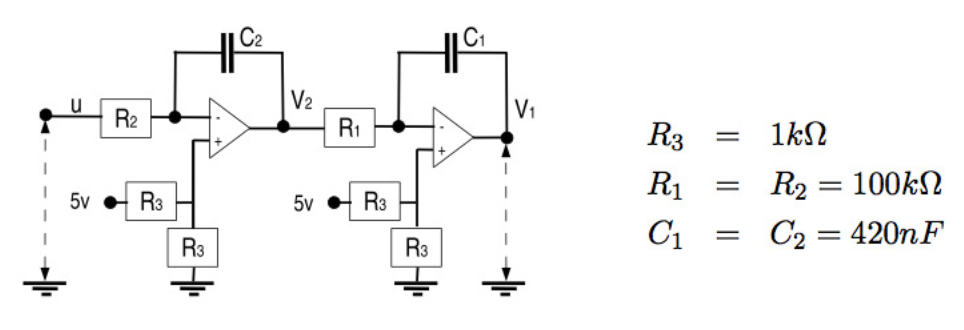
\includegraphics[width=0.8\textwidth]{Imatges/circuit_scheme.png}
\caption{Esquemàtic del doble integrador instal·lat a la placa \label{fig:doble_int_scheme}}
\end{figure}

\begin{table}[ht]
\begin{center}
\begin{tabular}{l|l}
Arduino & Doble Integrador\\
\hline
5v & 5v (LM358N power)\\
IOREF & 5v (voltage divider input)\\
GND & GND\\
A5 & $V_1$ DI output voltage\\
A4 & $V_2$ DI output voltage\\
D6 & u (PWM)
\end{tabular}
\caption{Taula de connexions entre el doble integrador i ports de l'Arduino \label{tab:con_DI_Ard}}
\end{center}
\end{table}

\newpage %Per no tallar el paragraf amb les figures superiors
Finalment, sobre el \textit{DI} només queda comentar el model matemàtic d'aquest. Desenvolupant les equacions de la dinàmica del circuit electrònic de la figura \ref{fig:doble_int_scheme} s'arriba a les equacions \eqref{eq:V1} i \eqref{eq:V2}. A partir d'aquestes equacions i dels valors numèrics de la figura \ref{fig:doble_int_scheme} s'arriba al model matemàtic del doble integrador que s'utilitza, expressat com \eqref{eq:DI_model_1}, \eqref{eq:DI_model_2} i amb els valors de \eqref{eq:DI_values} per les matrius del sistema de la planta .

\begin{eqnarray}
\dot{V_1} = - \frac{u}{R_2 C_2}\label{eq:V1} \\
\dot{V_2} = - \frac{V_2}{R_1 C_1}\label{eq:V2}
\end{eqnarray}

\begin{equation}\label{eq:DI_model_1}
\begin{bmatrix}
\dot{x_1}\\
\dot{x_2}
\end{bmatrix}
=
A_g
\begin{bmatrix}
x_1\\
x_2
\end{bmatrix}
+
B_g
u
\end{equation}

\begin{equation}\label{eq:DI_model_2}
y = C_g
\begin{bmatrix}
x_1\\
x_2
\end{bmatrix}
+ D_g
\end{equation}

\begin{equation}\label{eq:DI_values}
A_g = \begin{bmatrix}
0 & -23.8095\\
0 & 0
\end{bmatrix}
~~
B_g = \begin{bmatrix}
0 \\
-23.8095
\end{bmatrix}
~~
C_g = \begin{bmatrix}
1 & 0
\end{bmatrix}
~~
D_g = 0
\end{equation}

\newpage
\section{Metodologia}

En aquesta assignatura es treballa directament amb la planta a controlar i l'Arduino que és la que porta el control d'aquesta. Ara bé, abans d'implementar el control primer s'han de fer les simulacions pertinents. A més, en haver-se incorporat el codi de control en l'Arduino, s'ha de comprovar que aquest s'està duent a terme de forma correcte. Aquesta metodologia de treball és du a terme en cadascun dels tipus de control que es duen a terme en el treball. Tot seguit s'explica en detall quines accions i programari s'utilitza per fer-ho.

El primer és dur a terme la simulació del conjunt planta-controlador. Aquesta es fa amb la \textit{toolbox} \texttt{Simulink} havent fet els càlculs previs amb \texttt{Matlab}, tals com matrius d'alguns sistemes o valors dels controlador. En les simulacions s'extreuen les dades que es creguin convenients per tal d'esser analitzades, tant per comprovar si el sistema es controlat teòricament amb precisió, com per esser contrastades després amb les dades reals.

En tenir el sistema simulat i amb un controlador adient s'ha de procedir a implementar aquest a través de l'Arduino. Per fer-ho s'han de transformar el conjunt de blocs de simulació a equacions i codi. Aquesta tasca és més complicada del que sembla, aquí es demostra com de clars es tenen els coneixements i és molt fàcil equivocar-se en algun punt, tot i ser un simple detall.

Finalment s'ha de comprovar el bon funcionament del control. Per dur a terme aquesta fase el primer és tenir alguna sortida de dades del sistema real. En aquest cas, s'utilitza el \texttt{Serial Port} de l'Arduino on a través de les funcions \texttt{Serial.print} i \texttt{Serial.println} esdevenen sortides del que es desitgi. Per l'estudi en qüestió s'envien les variables que intervenen en el sistema al \texttt{Serial Port} com són: les variables d'estat $V_1$ i $V_2$, la referència, l'acció de control $u$ i altres variables que poden ser importants segons el control que es faci. Al treure les dades pel \texttt{Serial Port}, si s'envien seguint cert patrons, poden ser llegides i plotejades \textit{online} amb el programa \texttt{KST} per exemple, o també poder ser emmagatzemades en un fitxer per després ser analitzades amb \texttt{Matlab}. Amb les dades plotejades es pot comprovar la precisió del control o comparar-les amb les dades extretes de les simulacions.

\paragraph{$ $}

\section{Repositori de la pràctica}\label{sec:github}
En aquest tipus de pràctiques és molt comú l'ús de molt codi. Per tant, posar tota la informació en els Annexos pot ser molt incòmode, tant a l'hora de provar-ho, com si es vol corregir alguna errada. Per això es creu que el més convenient és posar tots els fitxers de codi, incluint el \texttt{Tex} del pròpi informe, en la plataforma \texttt{GitHub}.

La URL del repositori d'aquesta pràctica és:

\url{https://github.com/lluissalord/Control-Double-Integrator.git}

En aquest repositori es troben els diferents codis Arduino, fitxers format \texttt{.m} de \texttt{Matlab}, juntament amb els models de \texttt{Simulink} i els fitxers i imatges necessaris per dur a terme l'informe.

\chapter{Control de la planta}

La planta d'estudi es pot arribar a controlar de diverses formes, portant totes elles a l'estabilitat. Algunes porten l'estat a la referència amb més imprecisió que d'altres, com es comprova al llarg del treball, però totes elles provoquen que la planta sigui estable, que és l'objectiu del control. En aquesta part del treball és pretén explicar com s'han duit a terme els diferents controls i les característiques de cadascun d'ells.

\section{Control continu}

El control més senzill que es pot arribar a fer és considerar que el conjunt del sistema, planta-controlador, és en temps continu. En aquest cas, el sistema tan sols requereix del bloc de la planta, que utilitza els valors de les matrius de l'equació \eqref{eq:DI_values}, i una realimentació d'estat $K$, tal que els pols de llaç tancat siguin de part real negativa o nul·la (només si es un pol simple). Aquest tipus de sistema és simula amb l'esquemàtic de la figura \ref{fig:cont_scheme}.

\begin{figure}
\centering
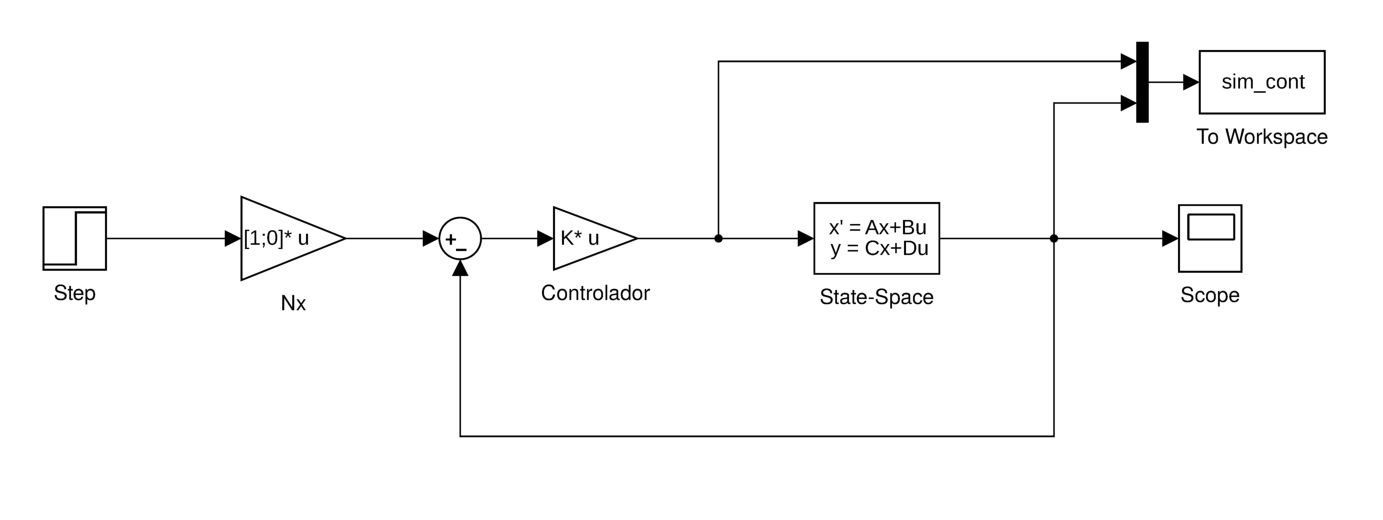
\includegraphics[width=0.8\textwidth]{Imatges/cont_sim_scheme.pdf}
\caption{Model de simulació del sistema amb control continu\label{fig:cont_scheme}}
\end{figure}

A banda del que s'acaba d'explicar, en la figura \ref{fig:cont_scheme} també apareixen una referència que es pretén seguir i el bloc $N_x$. Aquest permet que el sistema segueixi la referència donada. Per altra banda, també s'hi hauria d'incloure un bloc $N_u$ que multiplicaria la referència i es sumaria a l'acció de control $u$ a l'entrada de la planta, però com es veu en els càlculs de les equacions \eqref{eq:Nx_Nu}, $N_u$ és igual a zero. El sistema \eqref{eq:Nx_Nu} surt de desenvolupar els requisits \eqref{eq:req_N} per tal que es segueixi la referència. 

\begin{equation}\label{eq:req_N}
\left\{
\begin{array}{lr}
N_x r = x_r = x_ss \\
C_r X_ss = y_r = r
\end{array}
\right.
\end{equation}

\begin{equation}\label{eq:Nx_Nu}
\begin{bmatrix}
N_x\\
N_u
\end{bmatrix}
=
\begin{bmatrix}
A_g & B_g\\
C_g & 0
\end{bmatrix}^{-1}
\begin{bmatrix}
0\\
0\\
1
\end{bmatrix}
=
\begin{bmatrix}
1\\
0\\
0
\end{bmatrix}
\Rightarrow \left\{
\begin{array}{lr}
N_x = \begin{bmatrix}
1\\
0
\end{bmatrix} \\
N_u = 0
\end{array}
\right.
\end{equation}

Un cop es té el sistema montat de tal manera que aquest pugui seguir una referència, s'ha de buscar el controlador $K$ tal que porti el sistema a error zero. Per aconseguir-ho, existeixen diverses formes depenent de si es pensen imposar uns pols de llaç tancat determinats (per assignació de pols o amb la formula d'Ackermann) o si es pretén fer un control òptim a partir d'una funció de cost determinada (control \texttt{LQR}). En el cas d'estudi, s'utilitza la formula d'Ackermann imposant un pols de llaç tancat amb part real negativa o nul·la (només si és un pol simple).

Els pols que s'han d'imposar com s'ha dit abans han de ser uns que siguin de part real negativa o nul·la. Ara bé, en aquest sistema s'han d'escollir dos pols, per tant, aquests no poden ser de part real nul·la ja que farien el sistema inestable. Finalment, s'han escollit els pols $-5\pm20i$ que compleixen el requisit i que ha sigut proposat pel professor. 

Un cop escollits els pols tan sols queda aplicar la formula d'Ackermann. Aquesta dona el valor $K$ del controlador donats els pols desitjats i les matrius $A$ i $B$ del sistema. Al cap i a la fi, dona el mateix resultat que l'assignació de pols on s'iguala el polinomi característic desitjat amb $|z \mathbf{I} - (\mathbf{A_g} - \mathbf{B_g K})|$. La formula consisteix en l'equació \eqref{eq:Acker} on $p_d(A_g)$ és el polinomi característic desitjat amb el valor de la matriu $A_g$. En el \texttt{Matlab} la funció \texttt{acker} s'encarrega de fer aquests càlculs\footnote{Si es desitja llegir el codi \texttt{Matlab} utilitzat per fer tots els càlculs es pot trobar en el \texttt{GitHub} que es dona en la secció \ref{sec:github}}.

\vspace{-10pt}
\begin{equation}\label{eq:Acker}
K=(0\quad0\quad0\quad\dots\quad1)(\mathbf{A_g}\quad \mathbf{A_g B_g}\quad \mathbf{A_g^2 B_g}\quad \dots\quad \mathbf{A_g^{n-1} B_g})^{-1} p_d(A_g)
\end{equation}

Al tenir tots els valors es procedeix a dur a terme les simulacions. Les dades plotejades es mostren en la figura \ref{fig:cont_sim}. Aquí es pot veure com, en la simulació, s'aconsegueix estabilitzar la planta, tot i venir d'unes condicions inicials diferents a zero. Ara bé, aquesta simulació no s'adapta a la realitat, ja que l'Arduino envia l'acció de control de forma discreta i per tant el control no es correcte. Tot i que en aquest cas s'ha comprovat experimentalment que igualment es controla, tot i que no de la forma desitjada. Per tant, d'aquest tipus de control no se'n fa l'anàlisi experimental amb l'Arduino. 

\begin{figure}
\centering
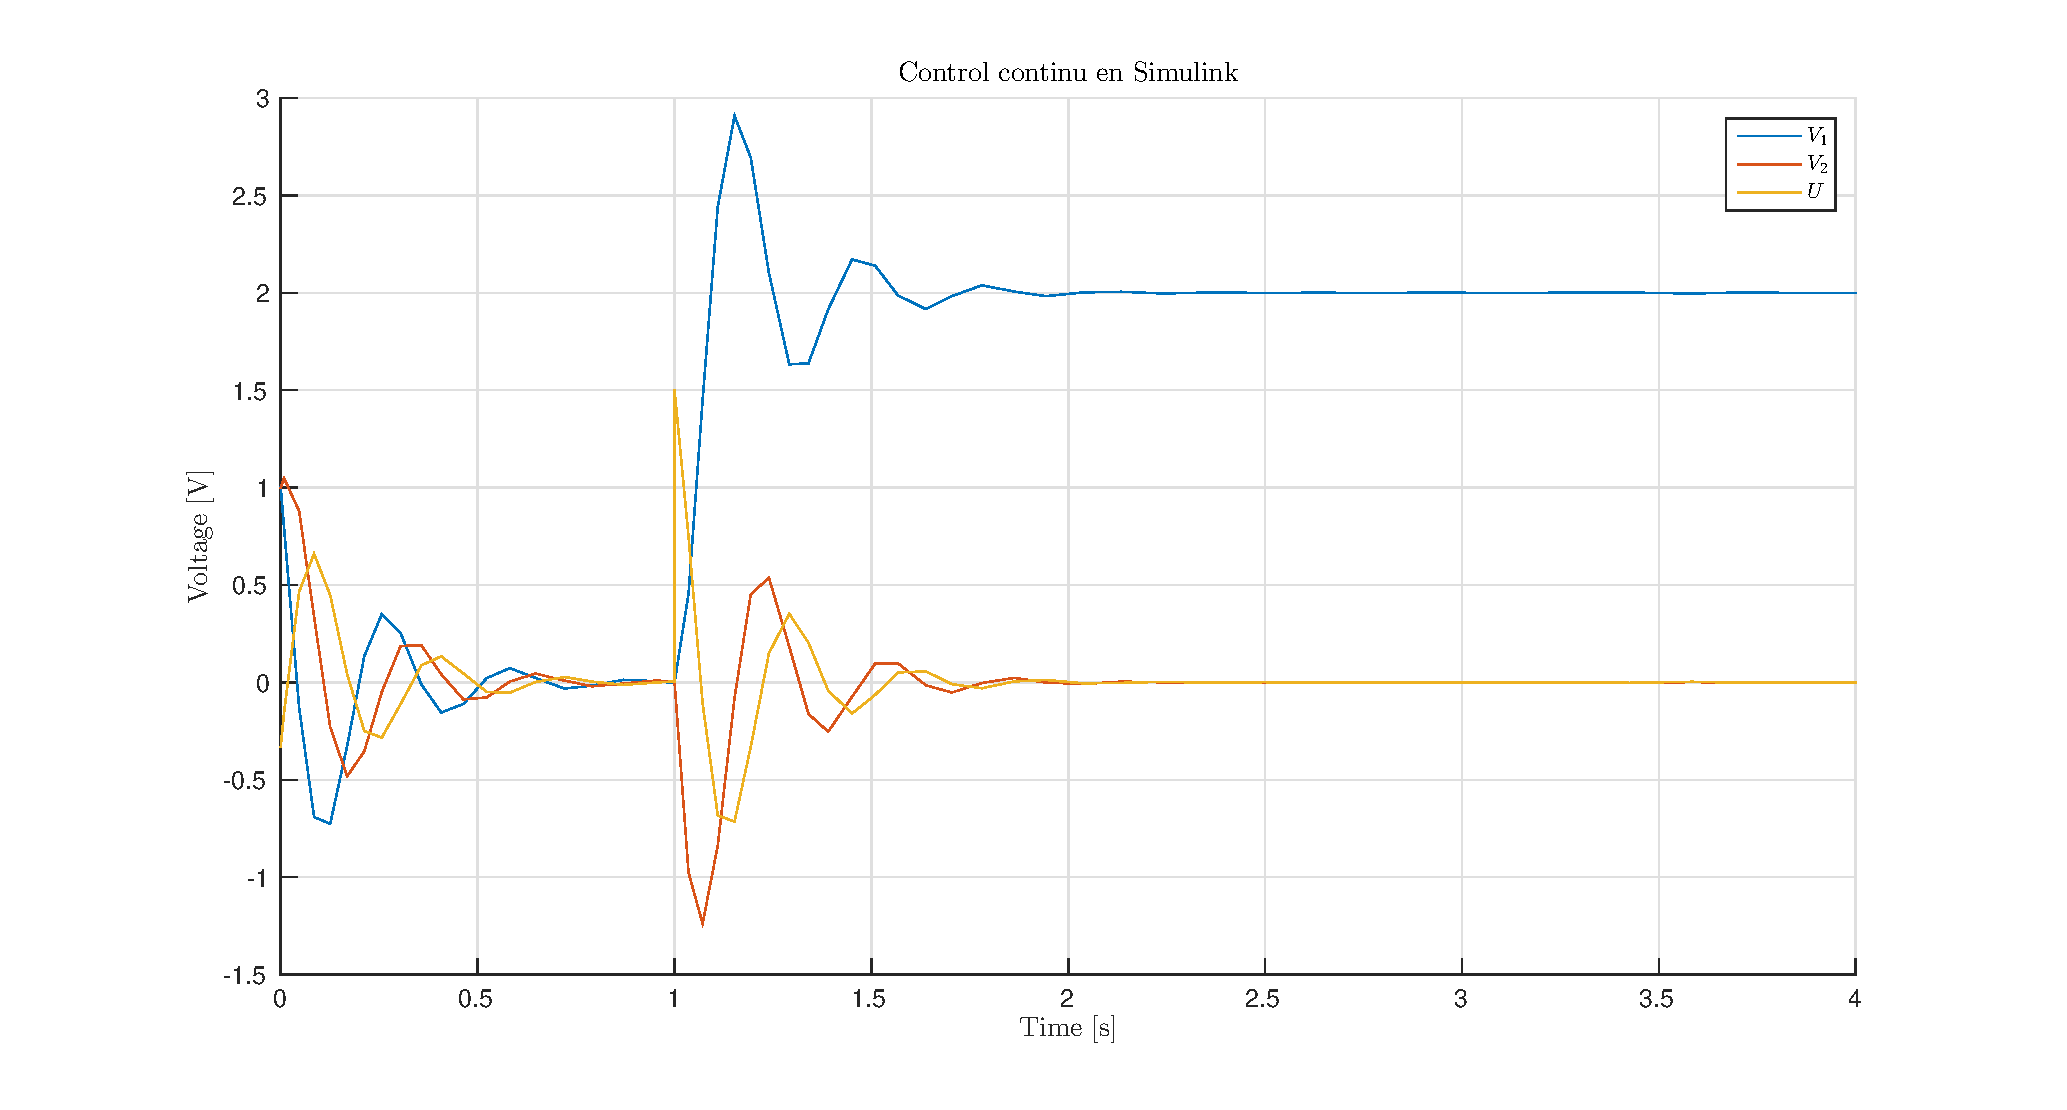
\includegraphics[width=0.8\textwidth]{Imatges/cont_sim.eps}
\caption{Dades de la simulació amb control continu\label{fig:cont_sim}}
\end{figure}

D'aquest cas no se'n fa un anàlisi en profunditat ja que no té especialment sentit físic. Només destacar, com es veu en la figura \ref{fig:cont_sim}, el fet que es demostra que una planta inestable, amb el controlador adequat por permetre l'estabilització del sistema.

\section{Control discret}

Com s'ha explicat en el cas del control continu, aquest no reflecteix la realitat, ja que el controlador (l'Arduino) funciona de forma discreta. Aquest llegeix les dades i fa els càlculs un cop cada cert temps, i envia el mateix valor del senyal durant aquest període.

El fet que es consideri el controlador discret no s'ha de confondre en que la planta funcioni de forma discreta. La planta és continua, l'únic que passa és que l'entrada, almenys la part que prové del controlador, és discreta i per tant el controlador s'ha d'adaptar a aquest tipus de funcionament. 

El primer que s'ha de fer és saber a quina freqüència treballa el controlador. En aquest cas, s'ha estipulat en l'enunciat un funcionament a $20 Hz$ (període de mostreig de $0.05 s$). Posteriorment, s'han de plantejar els pols de llaç tancat del sistema. Per simplificar, s'han escollit els mateixos que en el control continu, però discretitzats, que és fa aplicant l'equació \eqref{eq:pol_dis} als pols continus, sent $T_s$ el període de mostreig del controlador. Aplicant \eqref{eq:pol_dis} als pols continus, $-5\pm20i$, de l'apartat anterior, en resulten els pols discrets $0.4208\pm0.6553i$. El mòdul d'aquests pols és $0.7788$ es troben dins el cercle unitari, per tant, són estables. 

\begin{equation}\label{eq:pol_dis}
P_{dis} = e^{T_s P_{cont}}
\end{equation}
\vspace{10pt}


Per últim càlcul queda la $K$ del controlador, que es designa al llarg de treball com $K_{dis}$. Per tal d'aconseguir-ho també es pretén utilitzar la formula d'Ackermann \eqref{eq:Acker}, però no s'utilitzen les matrius $A_g$ i $B_g$, sinó les seves transformacions al sistema discret amb el període de mostreig $T_s$. Aquesta transformació es pot fer a través de la funció \texttt{c2d} del \texttt{Matlab}, on donades les matrius del sistema continu i el període de mostreig $T_s$ dona les matrius $\Phi$ i $\Gamma$ del sistema discret amb valors \eqref{eq:phi_gam}. Finalment, s'introdueixen les matrius $\Phi$ i $\Gamma$ i el període de mostreig a la funció \texttt{acker} i es té com a resultat el controlador $K_{dis} = \begin{bmatrix}
0.5398 & -0.6518
\end{bmatrix}$.\label{pag:trans_phi_gam}

\begin{equation}\label{eq:phi_gam}
\Phi=\begin{bmatrix}
1 &	-1,1905\\
0 & 1
\end{bmatrix} \;\;\;\;\;\;\; \Gamma=\begin{bmatrix}
0,7086\\
-1,1905
\end{bmatrix}
\end{equation}

Un cop és tenen tots els càlculs fets s'ha de procedir a dur a terme la simulació amb \texttt{Simulink}. El model de simulació és l'exposat en la figura \ref{fig:dis_sim_scheme}. A partir d'aquest, en surt el gràfic de la figura \ref{fig:dis_sim} que descriu la dinàmica del sistema amb el mateix tipus de referència que després s'utilitza en l'Arduino. Com es pot comprovar tendeix al valor de la referència en l'estacionari.

\begin{figure}[t]
\centering
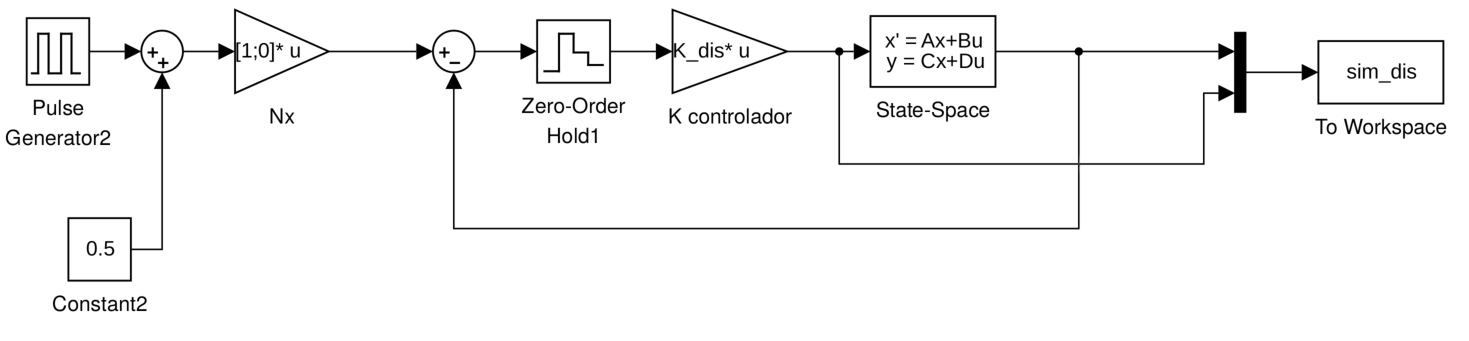
\includegraphics[width=0.8\textwidth]{Imatges/dis_sim_scheme.pdf}
\caption{Model de simulació del sistema amb control en discret\label{fig:dis_sim_scheme}}
\end{figure}

\begin{figure}[ht]
\centering
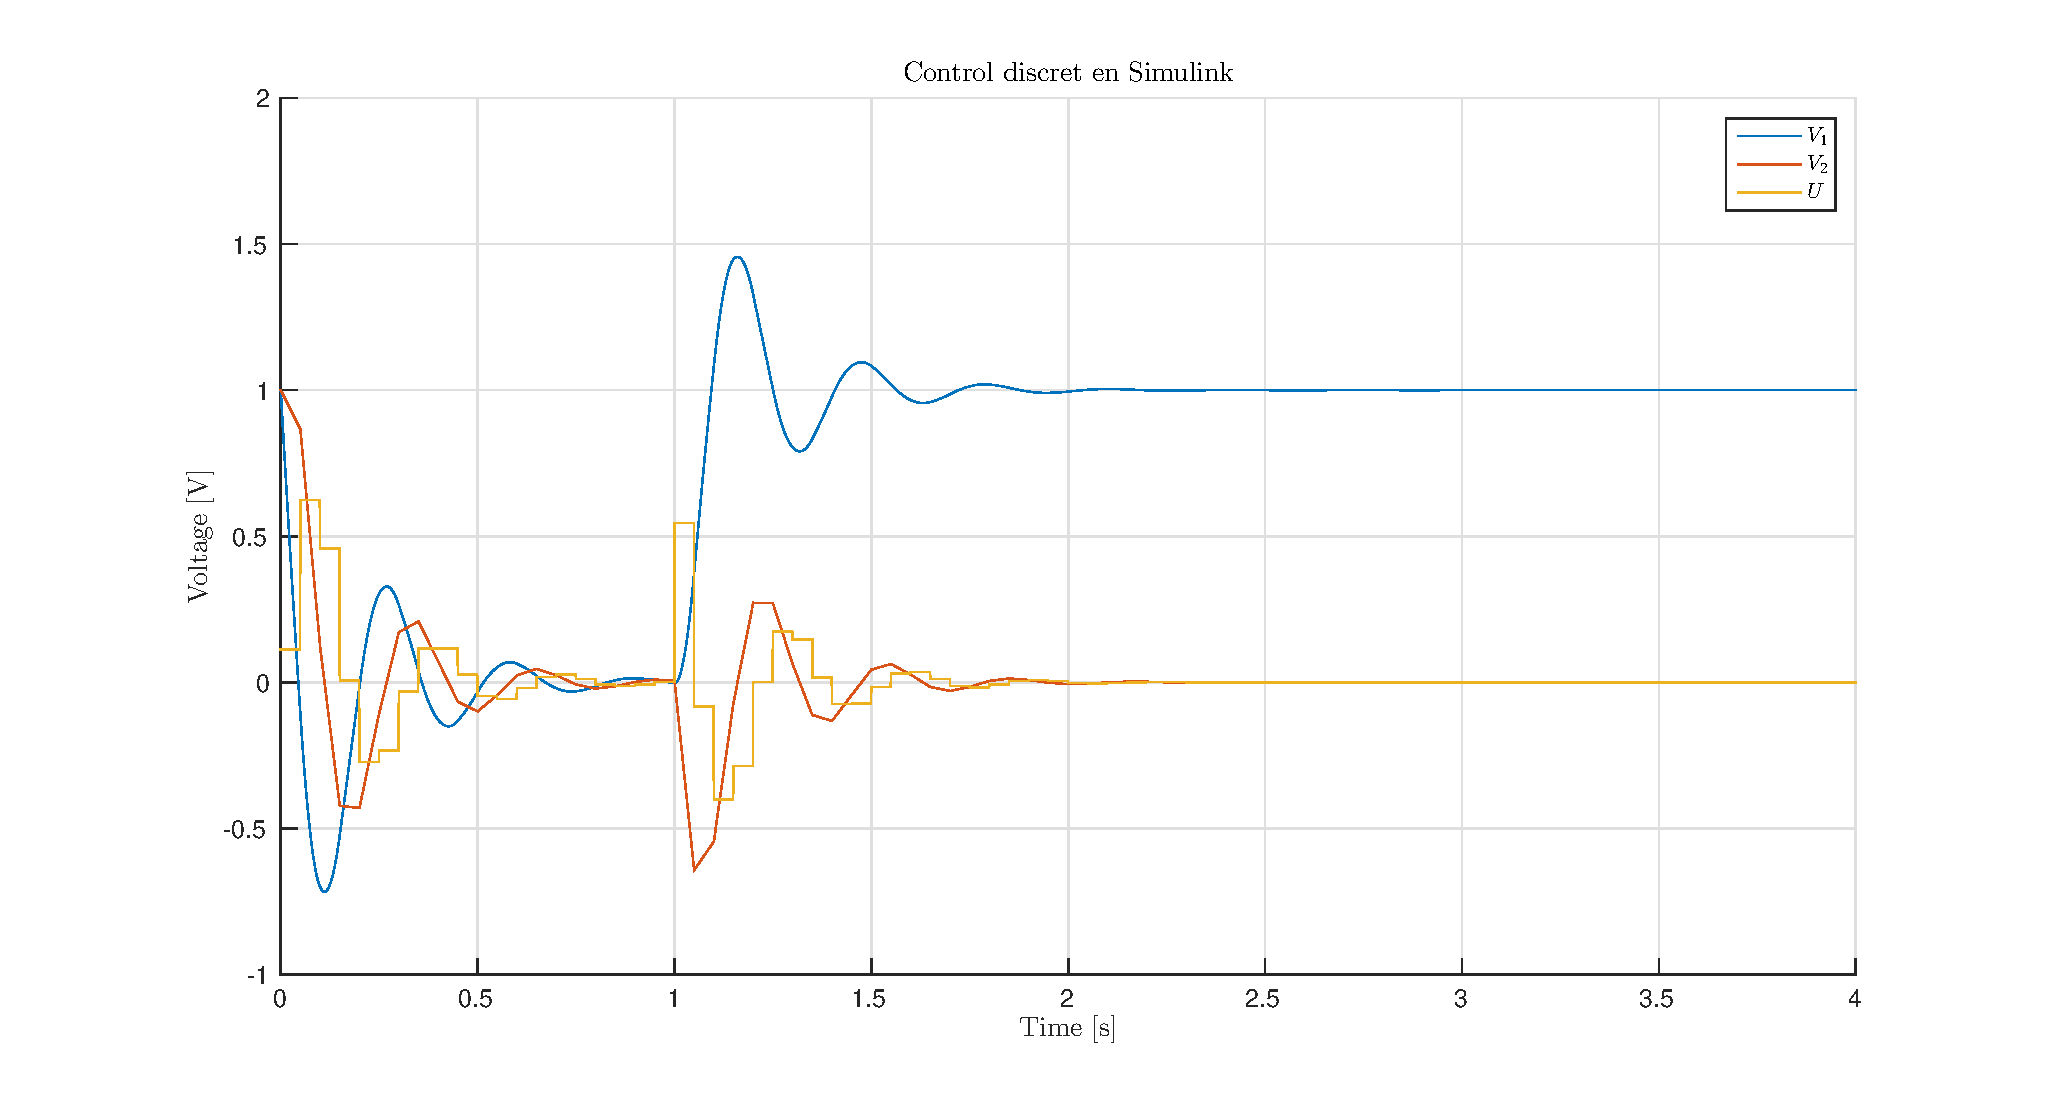
\includegraphics[width=0.8\textwidth]{Imatges/dis_sim.eps}
\caption{Dades de la simulació amb control discret\label{fig:dis_sim}}
\end{figure}

\newpage
Aquest al ser un cas més realista si que s'ha portat a fer les proves amb l'Arduino, per tal de veure si el comportament simulat i el real equivalen. A l'hora d'implementar el sistema en l'Arduino es pren la plantilla base de l'enunciat de la pràctica on tan sols falta l'algorisme de control y els valors de les constants. L'algorisme es basa en l'equació \eqref{eq:dis_u} on $V = \begin{bmatrix}
V_1\\
V_2
\end{bmatrix}$ i $r$ la referència que es pretén seguir.

\begin{equation}\label{eq:dis_u}
u=K_{dis} (N_x \cdot r - V) + N_u \cdot r
\end{equation}

Ara bé, s'han de tenir una sèrie de detalls en compte a l'hora d'implementar a l'Arduino:

\begin{itemize}
\item Al llegir les variables de l'exterior ($V_1$ i $V_2$) amb \texttt{analogRead} aquesta esta escalada entre 0 i 1023.
\item Al escriure pel \texttt{PWM} s'ha d'escalar entre 0 i 256.
\item Els voltatges estan \textit{offsejats} $2.5$ V a l'alça. Per tant, després de llegir i transformar a volts s'ha de restar $2.5$, per $V_1$ i $V_2$, i per $u$ abans d'enviar s'ha sumar $2.5$ per estar en referència absoluta.
\item S'ha de treballar amb variables tipus \texttt{float} o \texttt{double} per tal de fer els càlculs correctament.
\item La referència oscil·la entre $0.5$ i $1.5$ volts en lloc d'entre $1$ i $-1$ volts ja que sinó en algun moment s'arribava a la saturació i el funcionament no era del tot exacte.
\end{itemize}

Un cop passat a codi les equacions tenint en compte els punt anterior només s'ha d'afegir la part de codi que permet la lectura de les variables des de l'exterior. Això es du a terme a traves del \texttt{Serial Port} on amb la comanda \texttt{Serial.print} i \texttt{Serial.println} permet transmetre el que es desitgi. En aquest cas, s'envien les variables $V_1$, $V_2$, $U$ i la referència, totes aquestes en referència absoluta. Finalment, tan sols queda compilar i transferir el codi a l'Arduino.

A l'hora de comprovar que està passant a l'Arduino s'han arribat a utilitzar tres mètodes diferents segons el que es desitgi fer:

\begin{itemize}
\item Finestra del \texttt{Serial Port}, que es troba en la mateixa \texttt{IDE} de l'Arduino. Aquí es veu directament el que s'envia.
\item Programa \texttt{KST}, el qual si les variables s'envien amb un cert format es poden \textit{plotejar} en temps real.
\item A través de \texttt{Matlab}, un cop finalitzada l'escriptura de l'enviament de dades en un fitxer, importar les dades d'aquest.
\end{itemize}

D'aquests casos, tant el \texttt{KST} com el \texttt{Matlab}, requereixen de l'escriptura del que transmet el \texttt{Serial Port} en un arxiu de text. Això es pot fer utilitzant la comanda següent:

\texttt{cu -l /dev/ttyACM0 -s 115200 > nom\_arxiu.txt}

\vspace{10pt}
En cas del control discret les dades que s'han pogut extreure de l'Arduino són les que s'exposen en la figura \ref{fig:dis_all}. Com es pot observar, en aquest cas segueix molt bé la senyal, amb un petit soroll probablement degut al sensor a l'hora de llegir la senyal. Per tant, dur a terme una realimentació d'estat és un sistema de control que dona un bon resultat.

\begin{figure}
\centering
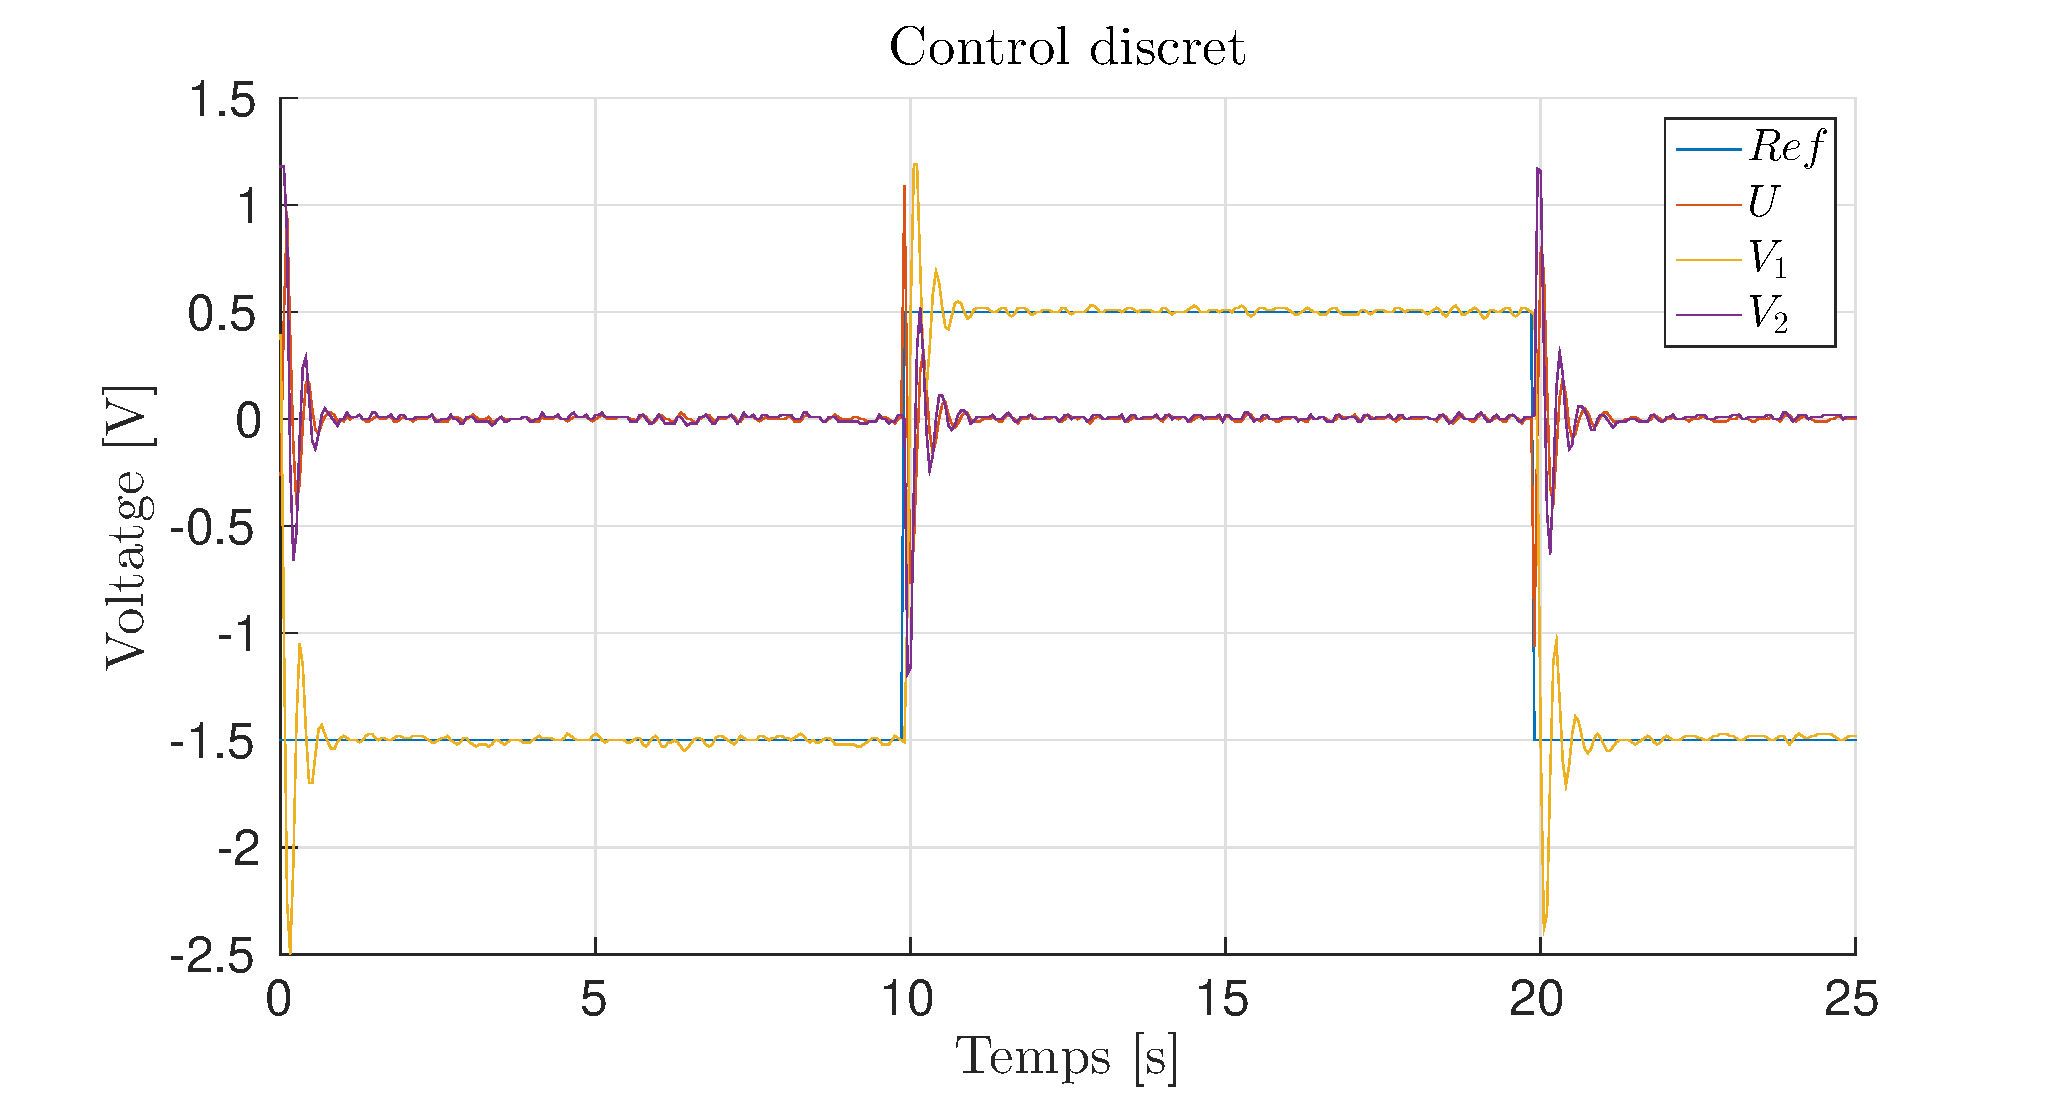
\includegraphics[width=0.8\textwidth]{Imatges/dis_all.eps}
\caption{Dades de l'Arduino amb control discret\label{fig:dis_all}}
\end{figure}

\section{Control amb observador}

Dur a terme una realimentació d'estat obliga a tenir un sensor per cadascun dels estats que es controlen. Aquest fet comporta un cost enorme en sensors. Per això, en molts cops es tendeix a fer el control de tot un sistema tan sols utilitzant un o uns pocs estats i per tant amb menys sensors. Per fer-ho s'utilitza un observador, que equivaldria a una simulació de la planta, però amb l'ús d'un o més dels estats reals per tal de portar sempre aquest observador al valor real.

Ara bé, no es pot implementar un control amb observador a qualsevol planta, aquestes han de complir que siguin observables, per tant que a partir de l'estat observat i l'acció de control es poden deduir tots els estats en un nombre finit de períodes $n$. Això es compleix si la matriu $W_o$ de l'equació \eqref{eq:observabilitat} és de rang $n$. En el cas d'estudi, el sistema es observable, i per tant, es pot dur a terme el control amb observador.
\vspace{-10pt}

\begin{equation}\label{eq:observabilitat}
W_o = \begin{bmatrix}
C\\
C A\\
C A^2\\
\vdots\\
C A^{n-1}
\end{bmatrix}
\end{equation}

La idea de l'observador és a partir del model de la planta, la sortida $y$ de la planta y l'acció de control $u$, estimar els estats de la planta i utilitzar aquesta estimació per realimentar el sistema, $u_k = -K_{dis}\cdot\bar{x}_k$. En aquest cas, s'ha considerat la matriu $C_g=[1 ~ 0]$, per tant, la sortida $y$ és $V_1$. Tenir en compte que l'observador, en la realitat, es troba en l'Arduino, per tant, és un sistema discret. Per això el model de la planta que s'utilitza en l'observador és el de la planta original passat a discret\footnote{El procés està explicat en la secció anterior a la pàgina \pageref{pag:trans_phi_gam}}, per tant, utilitza $\Phi$ i $\Gamma$.

Per altra banda, a l'hora d'escollir els pols, s'ha basat en utilitzar uns pols un poc més ràpids que els de la planta per a poder arribar al seu valor real, però no molt més per no amplificar el soroll que hi pugui haver. Per això, s'ha prés la part real dels pols de la planat i s'ha multiplicat per dos, sent així els pols de l'observador: $-10\pm20i$ en el pla S. 

Un cop escollits els pols, s'ha de procedir al càlcul de la $L$ de l'observador. Si es fes per assignació de pols, s'haurien d'igualar els pols, al polinomi $|z\mathbf{I}-(\mathbf{\Phi} - \mathbf{L C_g})|$. Ara bé, si observem en que es basava la formula d'Ackermann \eqref{eq:Acker}, es pot observar com si ara s'utilitza $\Phi^T$ i $C_g^T$ en lloc de $A_g$ i $B_g$ aquesta formula donaria com a resultat $L^T$. En aquest cas, s'ha utilitzat la formula de Ackermann de la forma anterior i ha donat com a resultat $L=\begin{bmatrix}
1,3446\\
-0,5985
\end{bmatrix}$

Com en tots els casos, un cop es tenen els valors de les matrius a utilitzar i les constants dels controladors, es procedeix a fer la simulació en \texttt{Simulink}. En aquest cas, el model queda expressat com en la figura \ref{fig:obs_sim_scheme}. El model de l'observador es basa en l'equació \eqref{eq:obs_model}. S'ha de tenir en compte el fet que la sortida de la planta a controlar és continua, per tant a l'hora d'utilitzar $y_k$, aquesta s'ha de discretitzar a la mateixa freqüència de treball del controlador per ser realista. A més, al voler tenir la informació de tots els estats, tot i ser $C_g=$[1 0] en la el bloc d'Espai d'Estats de la planta, s'ha donat una $C$ igual a la identitat i així poder llegir els estats, sent posteriorment multiplicat per $C_g$ per donar la sortida real.

\begin{equation}\label{eq:obs_model}
\bar{x}_{k+1} = \Phi \bar{x}_k + \Gamma u_k + L (y_k - C_g \bar{x}_k)
\end{equation}

\begin{figure}
\centering
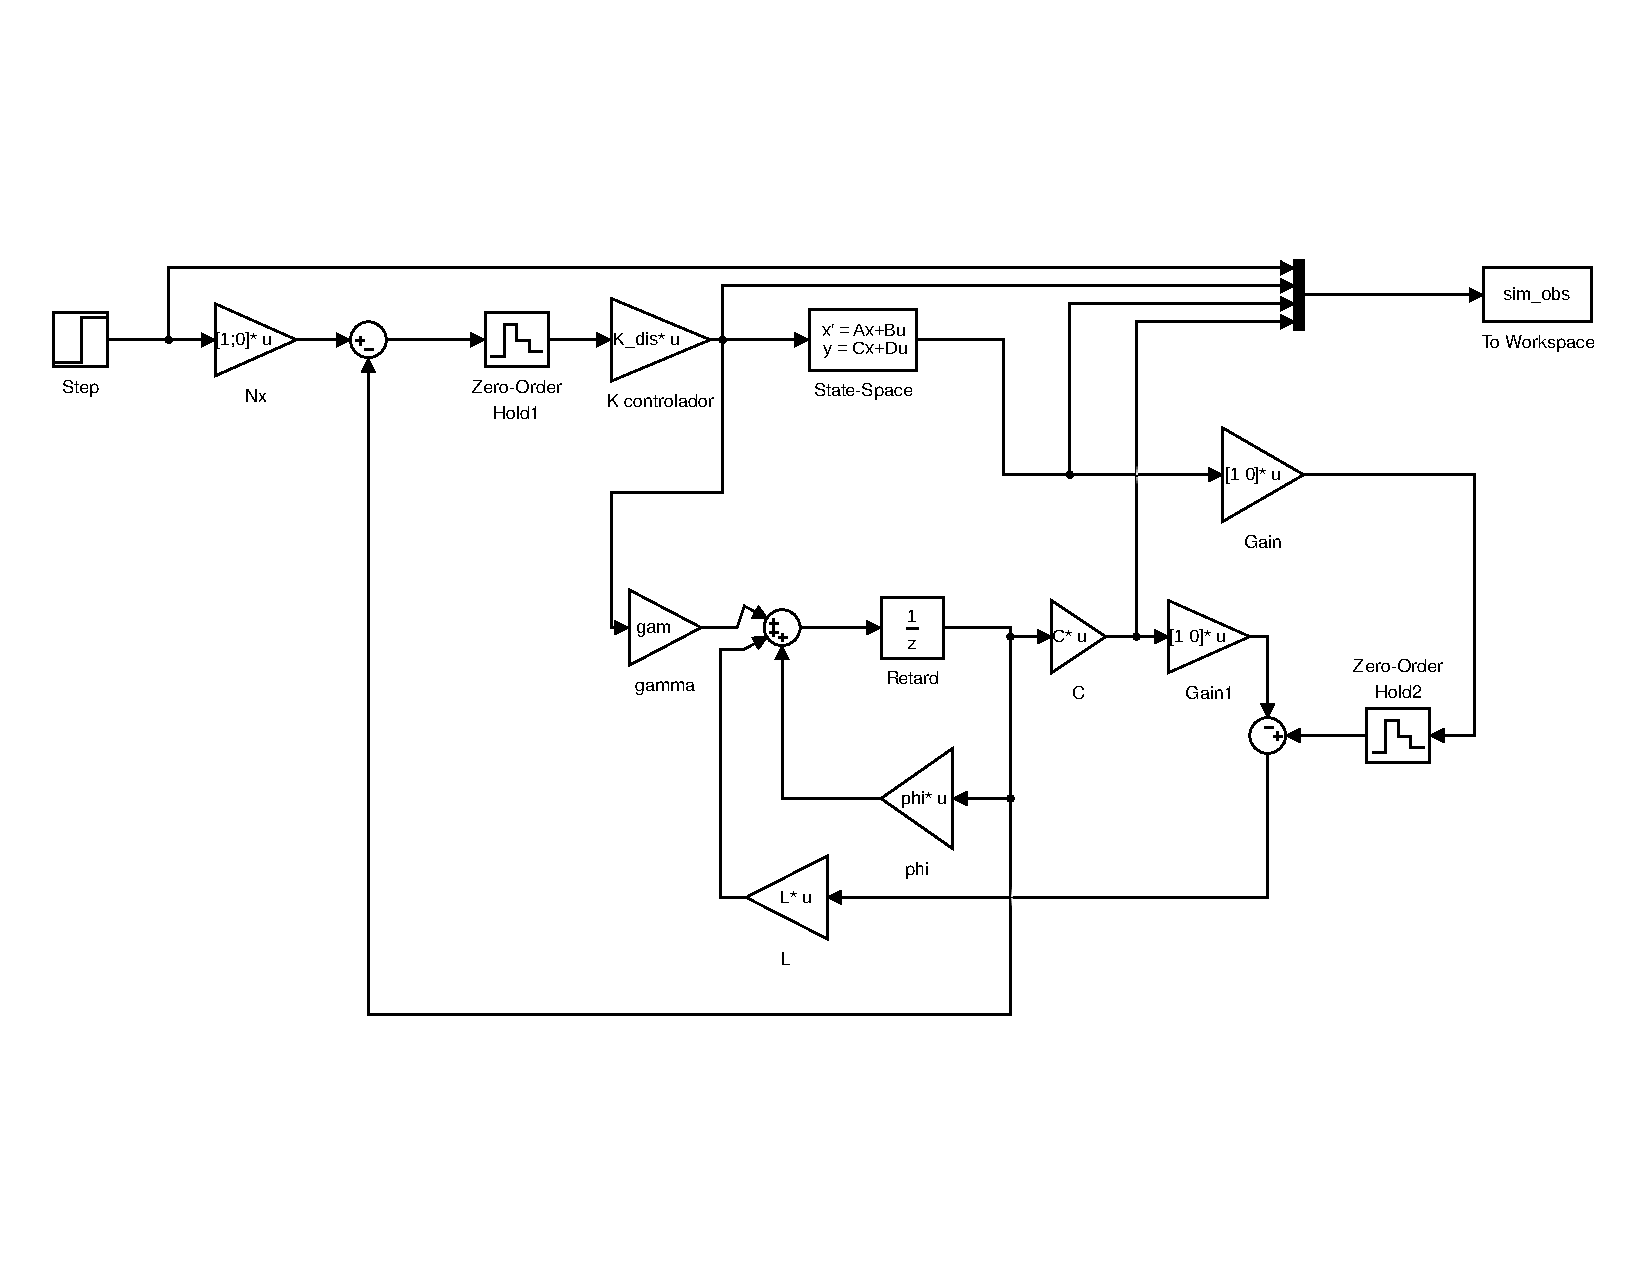
\includegraphics[width=0.8\textwidth]{Imatges/obs_sim_scheme.pdf}
\caption{Model de simulació del sistema amb control amb observador\label{fig:obs_sim_scheme}}
\end{figure}

Amb el model donat, el valor de $L$ calculat i les matrius $\Phi$ i $\Gamma$, el resultat de la simulació és el mostrat en la figura \ref{fig:obs_all_sim}. Aquí es comprova com és possible el control de la planta tan sols coneixent la sortida $V_1$ amb precisió.

\begin{figure}[h]
\centering
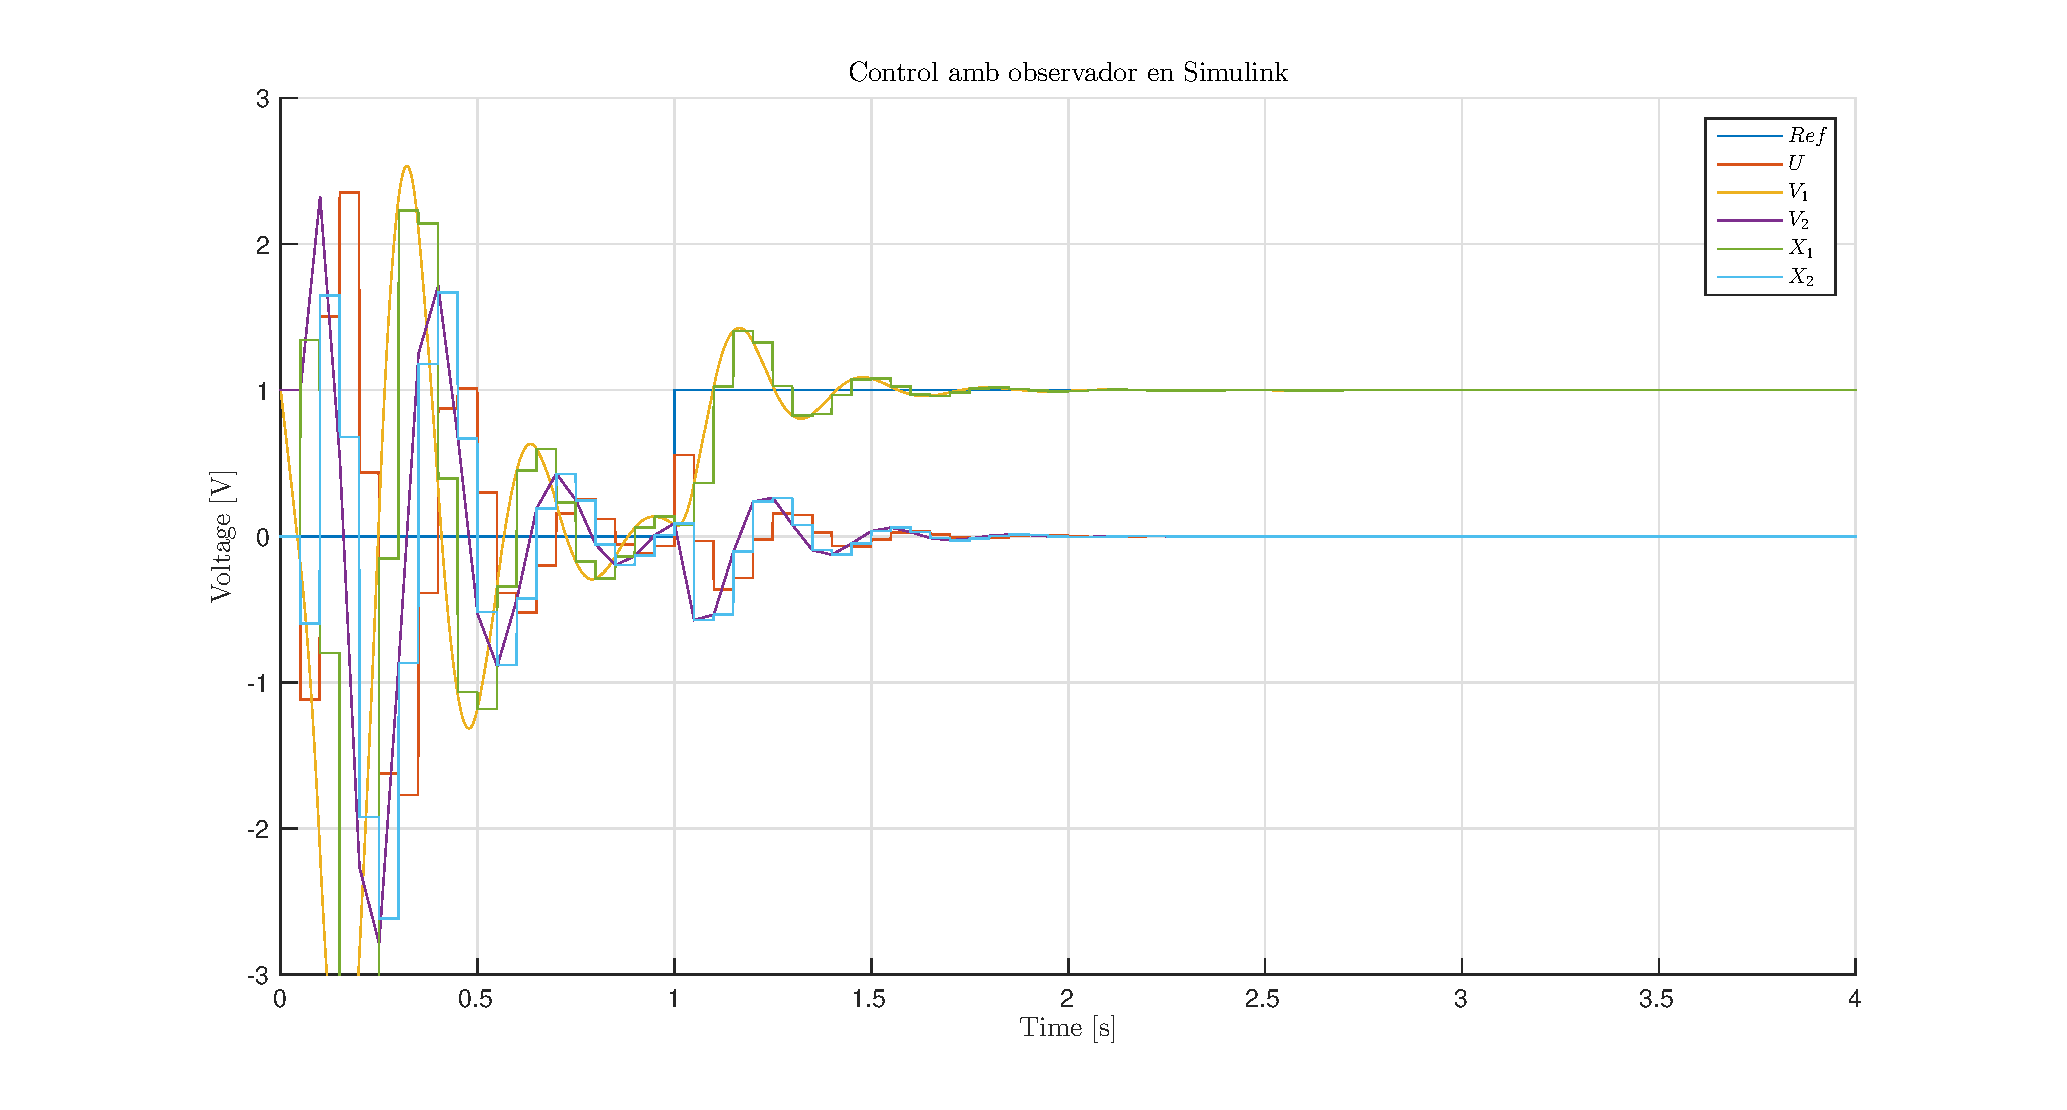
\includegraphics[width=0.8\textwidth]{Imatges/obs_all_sim.eps}
\caption{Dades de la simulació amb control discret\label{fig:obs_all_sim}}
\end{figure}

A l'hora d'implementar-ho en l'Arduino, el codi es basa en l'equació \eqref{eq:obs_model} i l'equació \eqref{eq:dis_u} adaptada al cas de l'ús de les variables d'observador que queda finalment com l'equació \eqref{eq:obs_u} sent $X=\begin{bmatrix}
X_1\\
X_2
\end{bmatrix}$ els estats de l'observador. Un detall a tenir en compte a l'hora d'escriure el codi és el fet que es necessari tenir una variable auxiliar on es guardin els valors de l'estat anterior per tal de poder fer els càlculs de forma adequada.

\vspace{-11pt}
\begin{equation}\label{eq:obs_u}
u=K_{dis} (N_x \cdot r - X) + N_u \cdot r
\end{equation}

Un cop s'ha implementat el codi, s'estudien les sortides per tal de veure si el control s'ha duit a terme de forma adequada. Les sortides en aquest cas són segons la figura \ref{fig:obs_all}. Es pot observar que el control és bastant acurat, tot i que amb un poc de soroll, i a més si es mira amb més detall, es pot veure com hi ha un petit \textit{offset} en tot el gràfic. Aquest fet és pot veure més en detall en la figura \ref{fig:obs_offset}. Per poder arribar a solucionar aquest problema una solució adequada és el control amb refús de pertorbacions constants.

\begin{figure}[h]
\centering
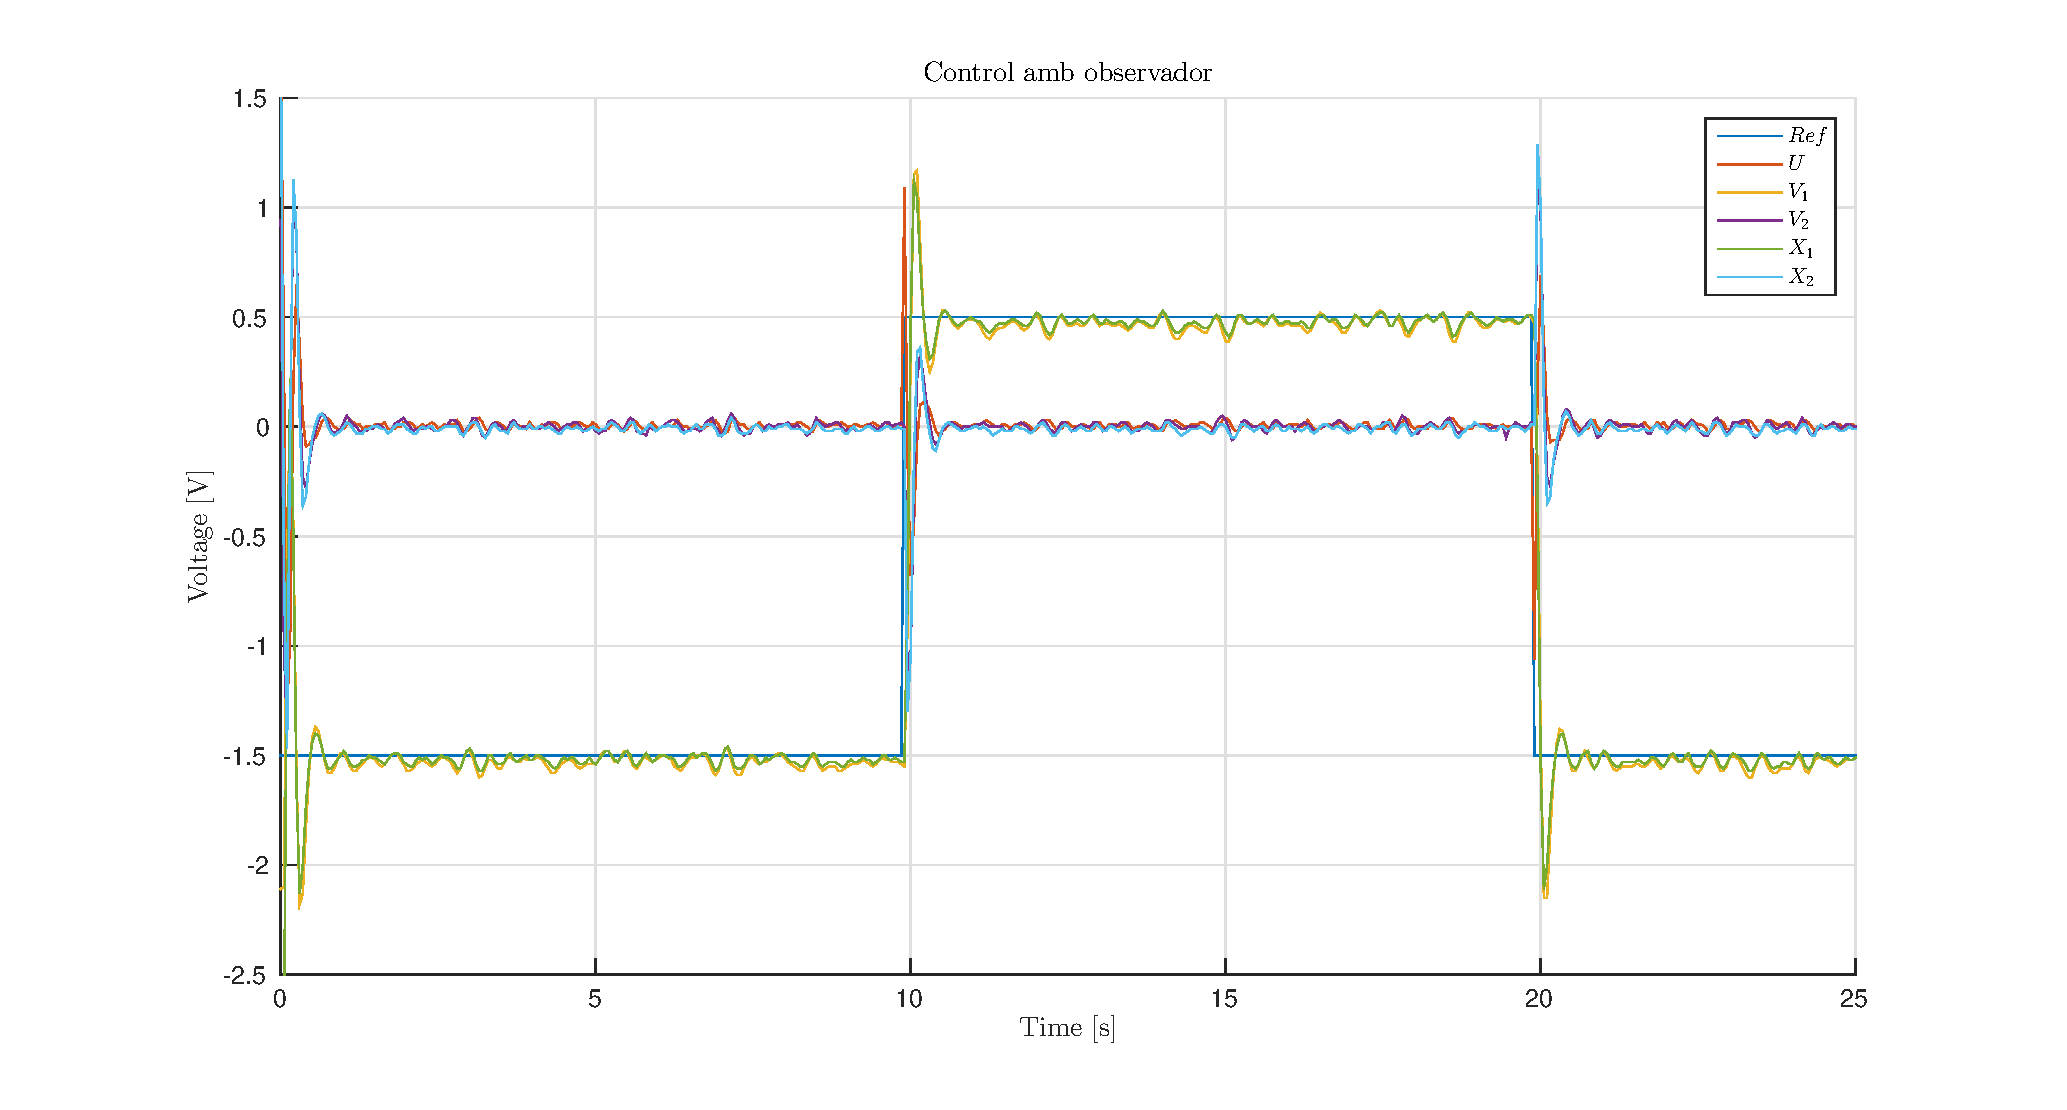
\includegraphics[width=0.8\textwidth]{Imatges/obs_all.eps}
\caption{Dades de l'Arduino amb control amb observador\label{fig:obs_all}}
\end{figure}

\begin{figure}[h]
\centering
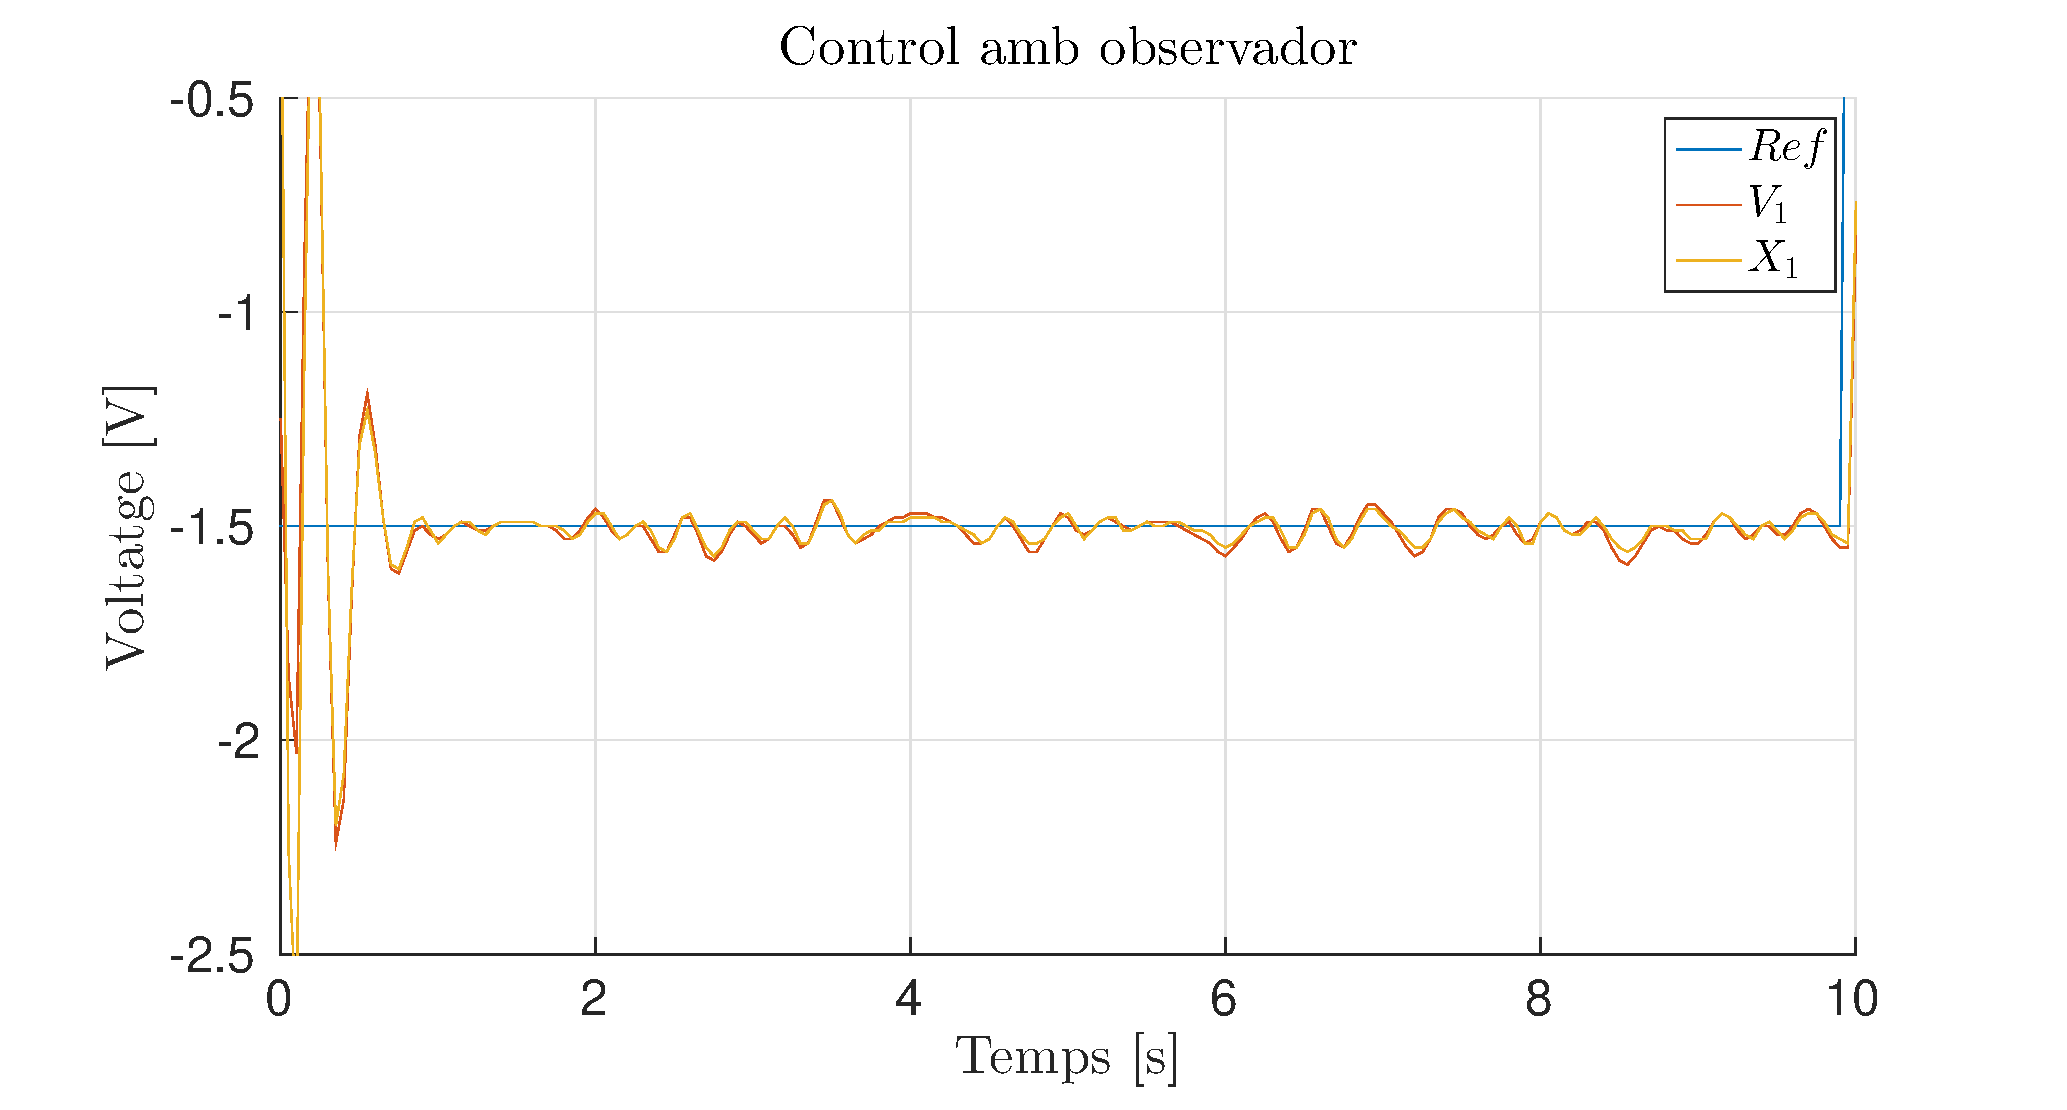
\includegraphics[width=0.8\textwidth]{Imatges/obs_offset.eps}
\caption{Detall de l'\textit{offset} del control amb observador\label{fig:obs_offset}}
\end{figure}

\section{Control amb refús de pertorbació}

El control amb refús de pertorbacions d'un determinat tipus de soroll també es pot entendre com un control per seguir una referència d'aquest mateix tipus. Realment, el que s'aconsegueix amb aquest tipus de control és que si l'error que s'està donant és de la forma que es pretén refusar o seguir, doncs s'aconseguix de forma perfecta. Per això, és pretén estimar la pertorbació $w$ i aquesta compensar-la amb l'estimació $\bar{w}$, on s'intenta aconseguir $\bar{w}=w$.

La base teòrica d'aquest control és estimar $w$, per fer-ho s'ha de modelar segons \eqref{eq:pert_cont} on $F^d$ i $C^d$ són les matrius que modelen la pertorbació i $x^d$ els estats. 

\begin{equation}\label{eq:pert_cont}
\left\{
\begin{array}{lr}
\dot{x}^d = F^d x^d\\
w=C^d x^d
\end{array}
\right.
\end{equation}

Això seria pel cas continu, ara bé, en aquest cas, l'observador ha d'estar en discret, per tant, s'ha d'utilitzar $\Phi^d=e^{F^d T_s}$ sent el model \eqref{eq:pert_dis}.

\begin{equation}\label{eq:pert_dis}
\left\{
\begin{array}{lr}
\dot{x}^d_k = \Phi^d x^d_k\\
w_k=C^d x^d_k
\end{array}
\right.
\end{equation}

Un cop modelada la pertorbació $w_k$\footnote{S'entén per $w_k$ l'estimació $\bar{w}$ de la pertorbació $w$ en discret. Aquesta nomenclatura és utilitzada al llarg de l'informe.}, aquesta s'ha d'incorporar al model general de tal manera que queda de la forma \eqref{eq:pert_model} que es pot reescriure amb forma matricial com \eqref{eq:pert_model_mat}

\vspace{-19pt}
\begin{equation}\label{eq:pert_model}
\left\{
\begin{array}{lr}
x_{k+1} = \Phi x_k + \Gamma u_k + \Gamma_1 w_k\\
y_k=C x_k
\end{array}
\right.
\end{equation}

\begin{equation}\label{eq:pert_model_mat}
\left\{
\begin{array}{lr}
\begin{bmatrix}
x_{k+1}\\
x^d_{k+1}
\end{bmatrix} = 
\begin{bmatrix}
\Phi & \Gamma_1 C^d\\
0 & \Phi^d
\end{bmatrix} \begin{bmatrix}
x_{k}\\
x^d_{k}
\end{bmatrix} + 
\begin{bmatrix}
\Gamma\\
0
\end{bmatrix} u_k = \Phi_w \begin{bmatrix}
x_{k}\\
x^d_{k}
\end{bmatrix} + \Gamma_w u_k\\
y_k=\begin{bmatrix}
C & 0
\end{bmatrix} \begin{bmatrix}
x_{k}\\
x^d_{k}
\end{bmatrix} = C_w \begin{bmatrix}
x_{k}\\
x^d_{k}
\end{bmatrix}
\end{array}
\right.
\end{equation}

Al tenir l'observador amb l'estimació de la pertorbació, tan sols cal trobar el valor de $L$ per tal de controlar el sistema. Aquest càlcul es du a terme, al igual que amb l'observador normal, amb la formula d'Ackermann utilitzant aquest cop les matrius ampliades $\Phi_w$ i $C_w$. S'ha de tenir en compte a l'hora d'estructurar el sistema complerts que els estats $x_{k+1}$ s'utilitzen com sempre en la realimentació \eqref{eq:obs_u}, mentre que la sortida $w_k$ s'introdueix al sistema com a \textit{feedforward}. Per altra banda, el sistema queda definit per les equacions \eqref{eq:pert_model_glob}, que equivalen al model de \texttt{Simulink} de la figura \ref{fig:pert_sim}.

\begin{equation}\label{eq:pert_model_glob}
\left\{
\begin{array}{lr}
u_k=K_{dis} (N_x \cdot r - \bar{x}_{k}) + N_u \cdot r - w_k\\
\begin{bmatrix}
\bar{x}_{k+1}\\
\bar{x}^d_{k+1}
\end{bmatrix} = \Phi_w \begin{bmatrix}
\bar{x}_{k}\\
\bar{x}^d_{k}
\end{bmatrix} + \Gamma_w u_k + L (y_k - C_g \begin{bmatrix}
\bar{x}_{k}\\
\bar{x}^d_{k}
\end{bmatrix})
\end{array}
\right.
\end{equation} 

\begin{figure}[ht]
\centering
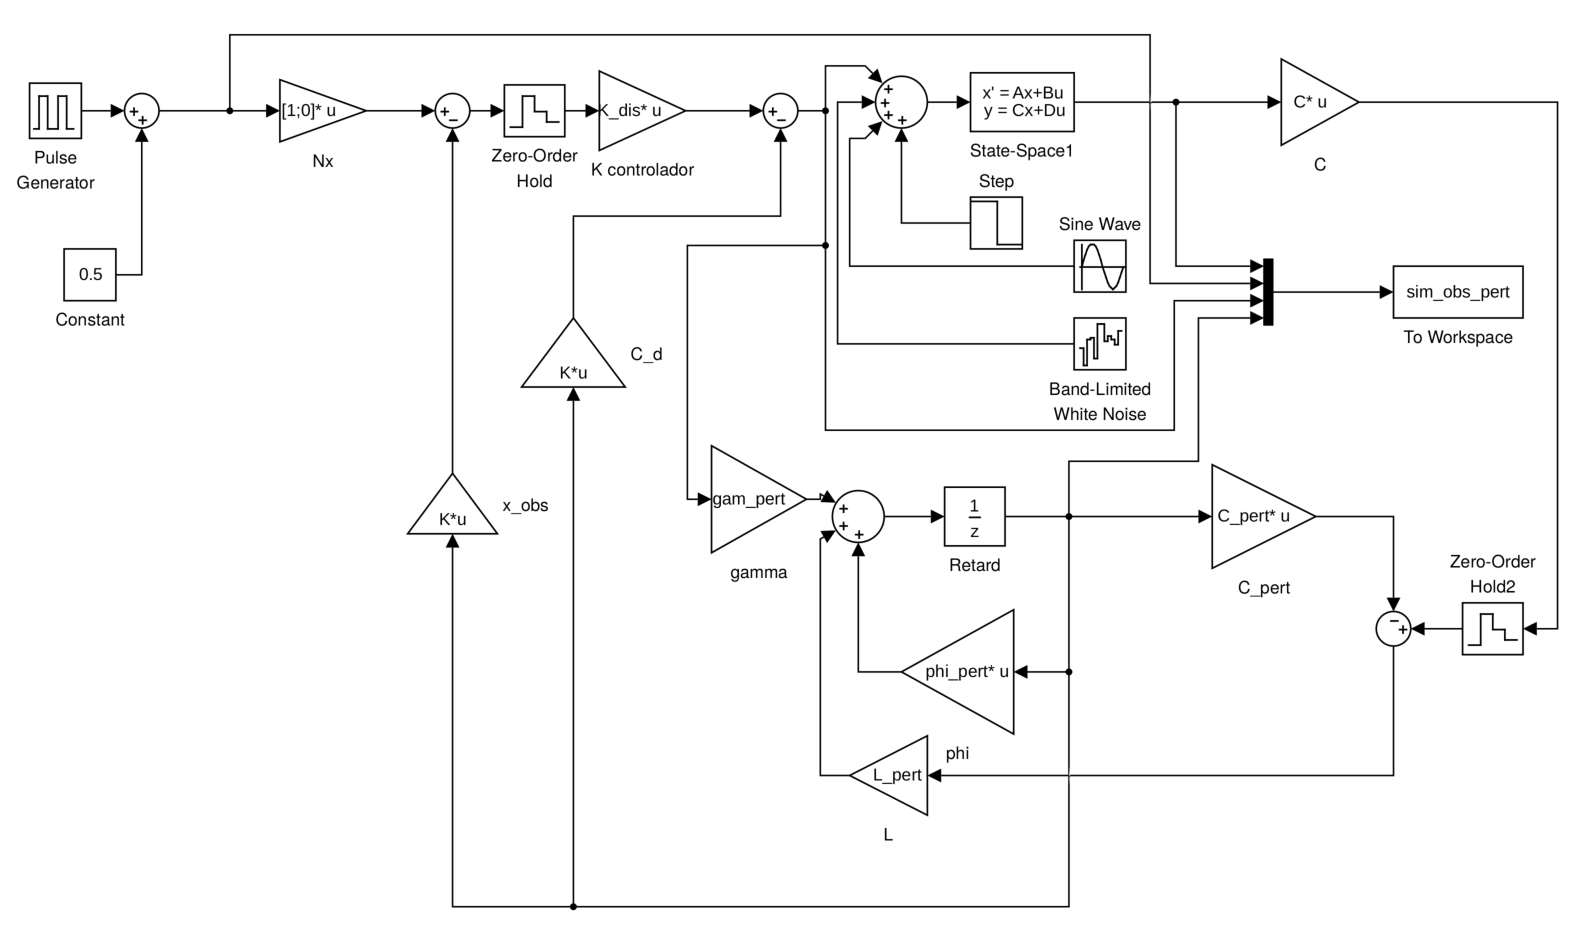
\includegraphics[width=0.8\textwidth]{Imatges/pert_sim.pdf}
\caption{Model de simulació del sistema amb control am refús de pertorbacions\label{fig:pert_sim}}
\end{figure}

D'aquest model de simulació per \texttt{Simulink}, cal comentar uns quants detalls.
\begin{enumerate}
\item S'han posat diferents tipus de pertorbacions, per comprovar com d'acurat és el refús, tot i que no s'apliquen tots en tots els gràfics. En cadascun dels gràfics s'especifica quin tipus de pertorbacions s'hi han aplicat.
\item Els blocs anomenats \texttt{phi}, \texttt{gamma} i \texttt{C\_obs}; corresponen a les matrius ampliades $\Phi_w$, $\Gamma_w$ i $C_w$.
\item Segons el tipus de pertorbacions que es pretén refusar, la dimensió de les matrius canvia. Ara bé, si es segueixen les equacions com s'han expressat al llarg del treball, les úniques que s'han de modificar segons la pertorbació són les de la realimentació d'estats observats i la del \textit{feedforward}, per tal d'utilitzar els estats corresponents.
\end{enumerate}

En aquest informe es pretén dur a terme el control amb refús de pertorbacions tant constants, com sinusoïdals. A continuació s'expliquen els passos que s'han seguit per aconseguir-ho.

\subsection{Pertorbació constant}

En el cas de les pertorbacions constants, el model que les defineix és \eqref{eq:pert_const}. Per tant, el model de l'observador queda com \eqref{eq:pert_const_model_mat}. Posteriorment, s'aplica la formula d'Ackermann resultant $L=\begin{bmatrix}
0.71467\\
-0.12109\\
0.00614
\end{bmatrix}$

\begin{equation}\label{eq:pert_const}
\left\{
\begin{array}{lr}
\dot{x}^d_k = x^d_k\\
w_k = x^d_k
\end{array}
\right.
\end{equation}

\begin{equation}\label{eq:pert_const_model_mat}
\left\{
\begin{array}{lr}
\begin{bmatrix}
x_{k+1}\\
w_{k+1}
\end{bmatrix} = 
\begin{bmatrix}
\Phi & \Gamma \\
0 & 1
\end{bmatrix} \begin{bmatrix}
x_{k}\\
w_k
\end{bmatrix} + 
\begin{bmatrix}
\Gamma\\
0
\end{bmatrix} u_k\\
y_k=\begin{bmatrix}
C & 0
\end{bmatrix} \begin{bmatrix}
x_{k}\\
w_k
\end{bmatrix}
\end{array}
\right.
\end{equation}

Aleshores, amb les matrius $\Phi_w$, $\Gamma_w$ i $C_w$ de \eqref{eq:pert_const_model_mat} i el vector $L$ calculat, amb l'ús de \eqref{eq:pert_model_glob} es procedeix a la simulació del model \ref{fig:pert_sim} amb \texttt{Simulink}.

En primer lloc es representa el model amb només la pertorbació d'un \textit{step}, de tal manera que sense el refús de pertorbacions la sortida es quedaria \textit{offsetejada} segons l'amplitud de l'\textit{step}\footnote{L'amplitud d'aquest \textit{step} és aproximadament l'\textit{offset} de la planta real observat en la figura \ref{fig:obs_offset}}. La figura \ref{fig:pert_ct_all_sim_pols_imag_no_sin} mostra els diferents valors d'aquest cas\footnote{Mencionar que la variable del gràfic anomenat $X_3$ és l'estimació $w_k$ del sistema.}. Com es comprova, la sortida es troba perfectament situada sobre la referència, per tant l'\textit{offset} no afecta amb aquest control.

\begin{figure}[ht]
\centering
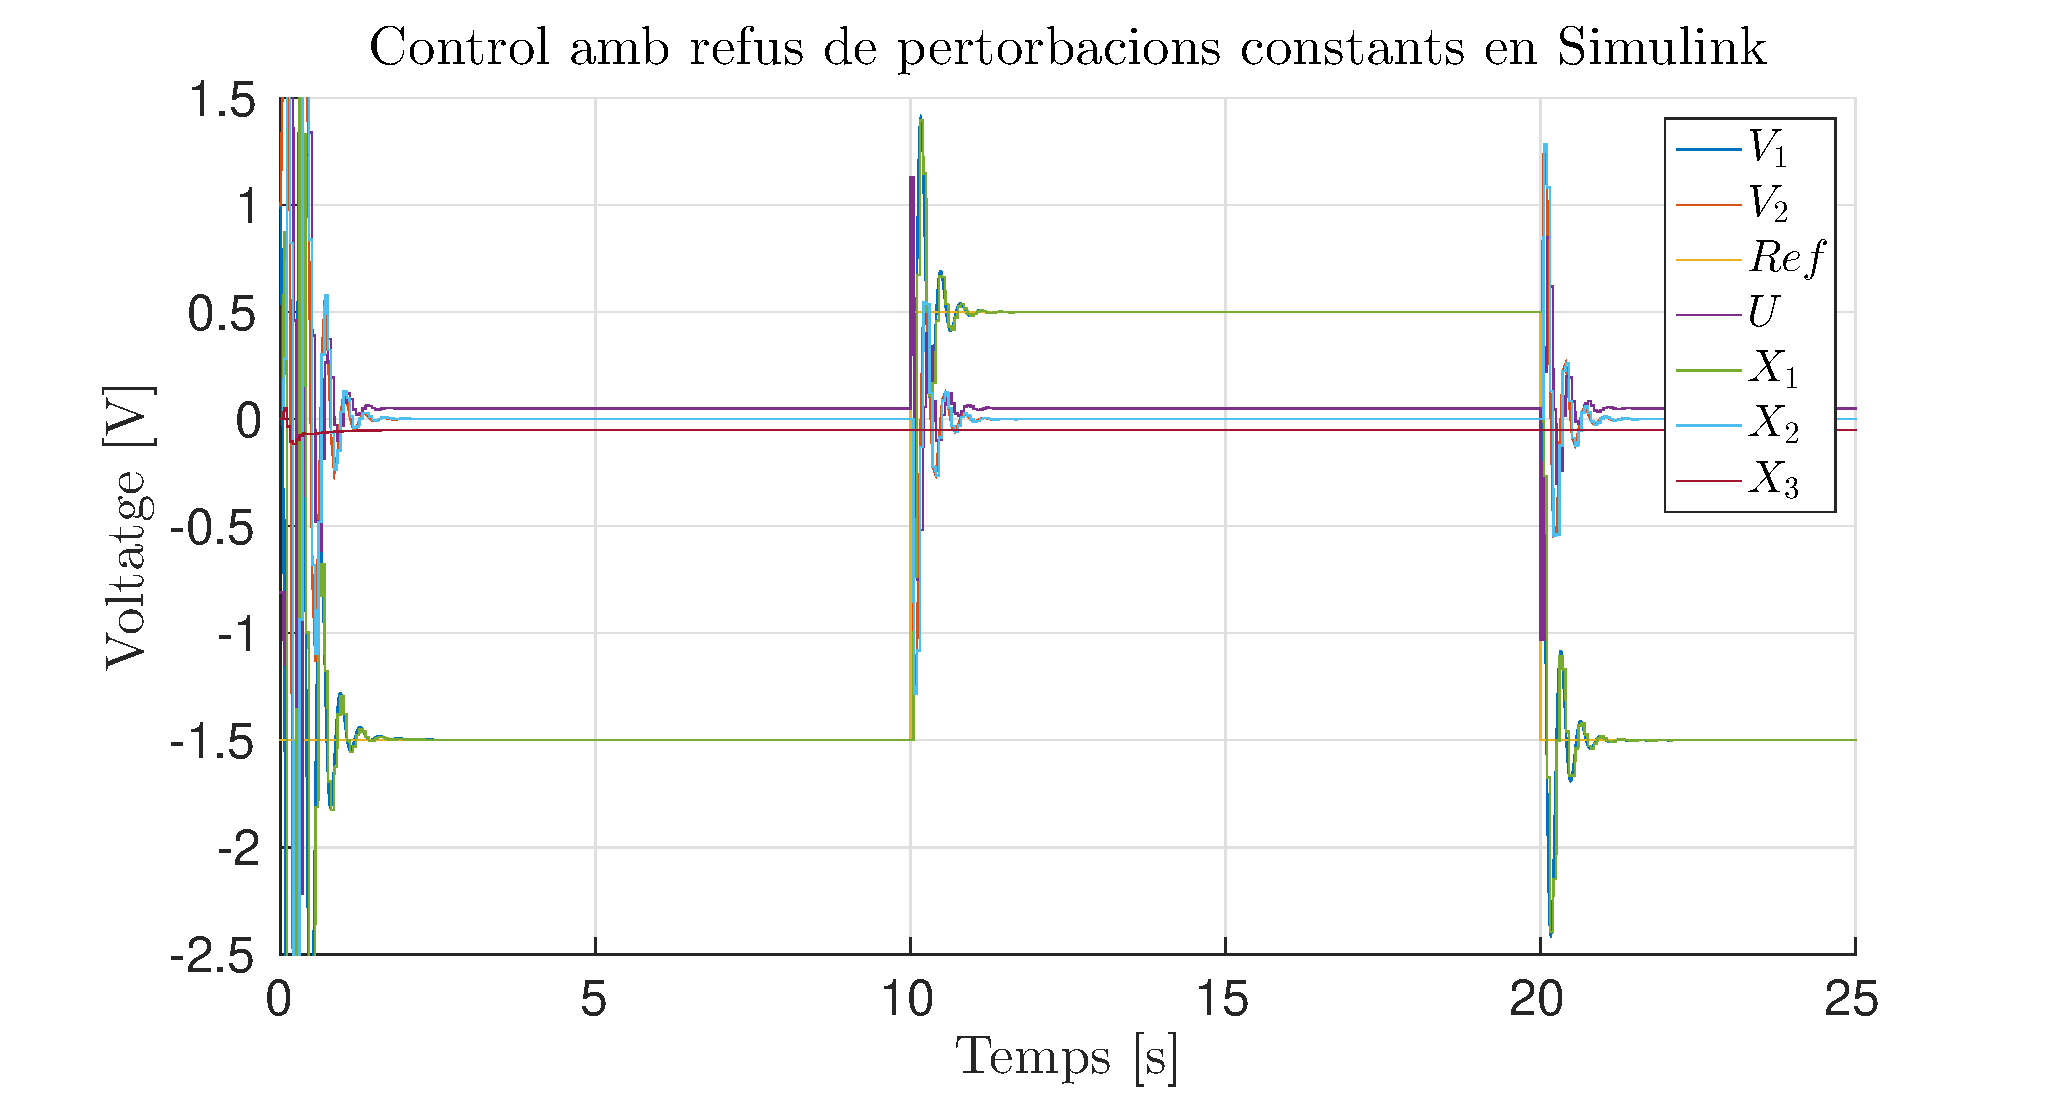
\includegraphics[width=0.8\textwidth]{Imatges/pert_ct_all_sim_pols_imag_no_sin.eps}
\caption{Dades de la simulació amb control amb refús de pertorbacions constants amb un \textit{step}\label{fig:pert_ct_all_sim_pols_imag_no_sin}}
\end{figure}

Per altra banda, es planteja veure que tal és el control si s'introdueix, a més, una pertorbació de tipus sinusoïdal\footnote{Més endavant s'expliquen les característiques d'aquesta sinusoïdal que és una aproximació del soroll a la planta real.}. Aquest és el cas de la figura \ref{fig:pert_ct_all_sim_pols_imag_sin}. Com es pot comprovar, aquest control no permet seguir de forma adequada senyals de tipus sinusoïdals, per tant, si es té un soroll d'aquest tipus aquest no és refusa, al menys amb aquest control.

\begin{figure}[ht]
\centering
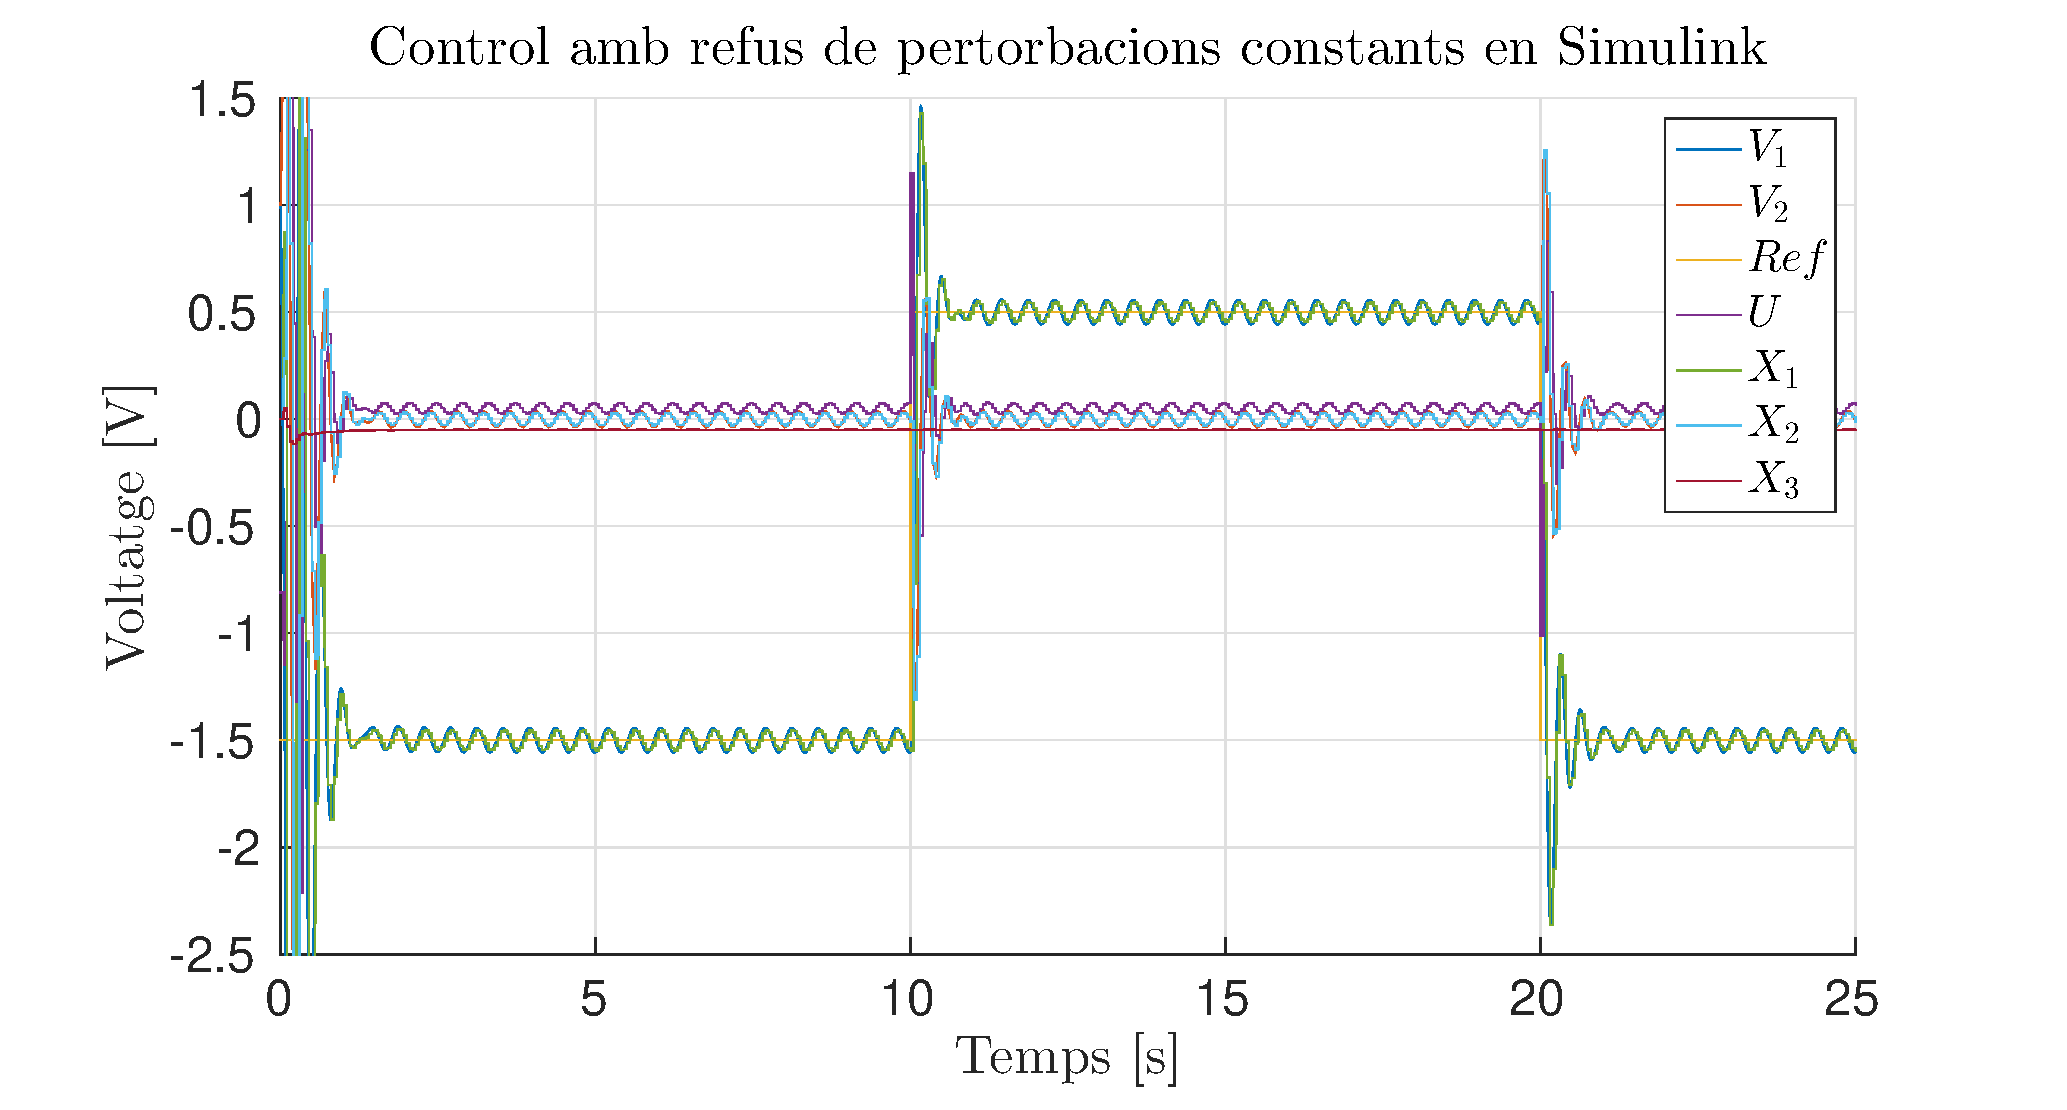
\includegraphics[width=0.8\textwidth]{Imatges/pert_ct_all_sim_pols_imag_sin.eps}
\caption{Dades de la simulació amb control amb refús de pertorbacions constants amb un \textit{step} i una sinusoïdal\label{fig:pert_ct_all_sim_pols_imag_sin}}
\end{figure}

Un cop s'ha comprovat la implementació en \texttt{Simulink} es procedeix a la implementació en l'Arduino. Tan sols s'han d'implementar les equacions \eqref{eq:pert_model_glob} amb les matrius $\Phi_w$ i $\Gamma_w$ calculades de \eqref{eq:pert_const_model_mat} i la $L$ calculada per Ackermann. A partir d'aquesta implementació en surt el gràfic \ref{fig:pert_ct_all_pols_imag} amb totes les dades que es poden extreure. Es pot veure, com aquest cop la sortida no té cap mena d'\textit{offset} respecte la referència que ha de seguir.

Ara bé, es cert que en les figures \ref{fig:obs_all} i \ref{fig:obs_offset}, on es pot veure l'\textit{offset} quan no hi ha refús de pertorbacions constants, no es molt notable aquest fet. Per tant, per comprovar que no fos casualitat que justament la placa no tingués \textit{offset} o que fos inapreciable, s'ha fet el test d'introduir el codi "\texttt{u=u+0.1}", després del càlcul però abans d'enviar-lo pel \texttt{PWM}. Amb això s'aconsegueix que estar segur que existeix una pertorbació constant i si la refusa significa que el control funciona de forma adequada. S'ha fet el test i ha funcionat a la perfecció.

\begin{figure}
\centering
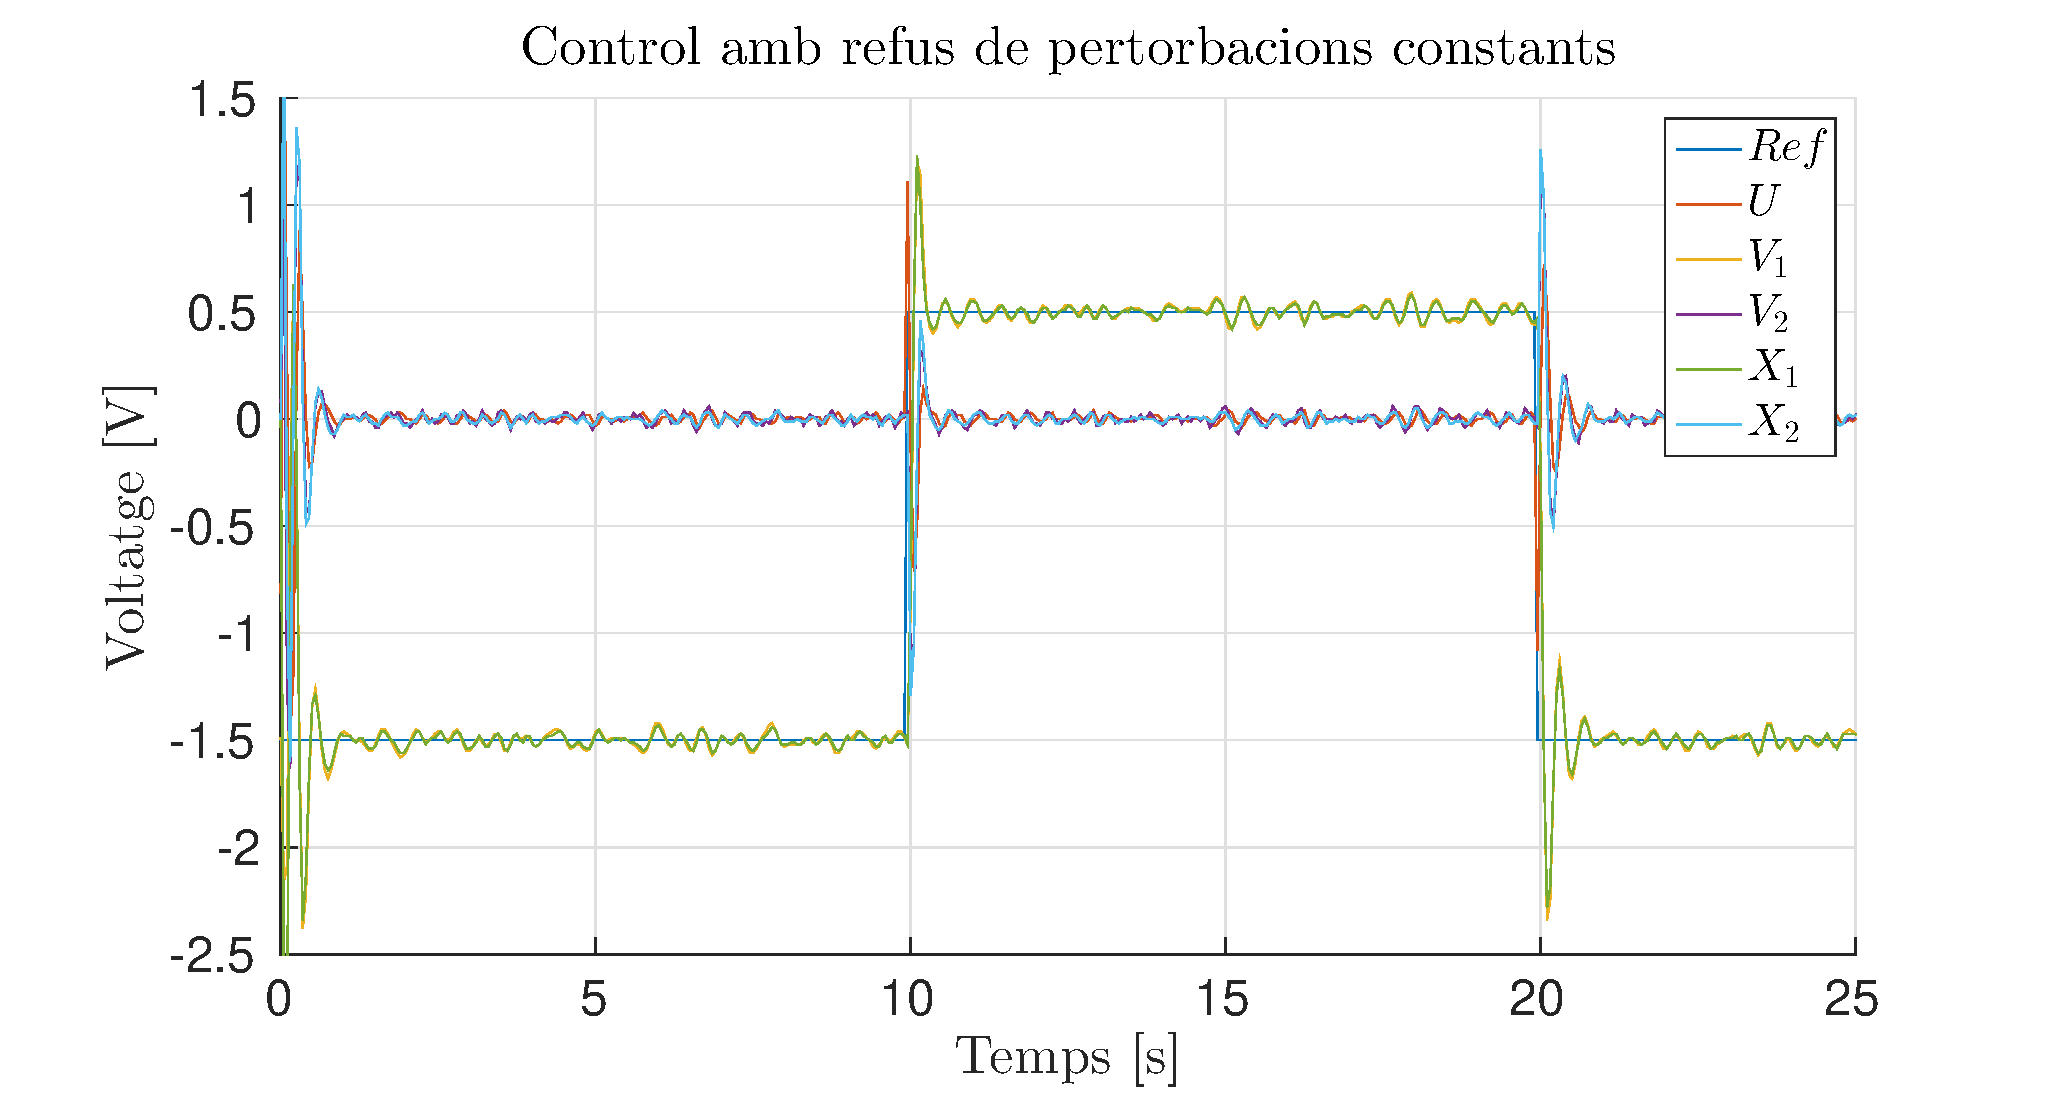
\includegraphics[width=0.8\textwidth]{Imatges/pert_ct_all_pols_imag.eps}
\caption{Dades de l'Arduino amb control amb refús de pertorbacions constants\label{fig:pert_ct_all_pols_imag}}
\end{figure}

\subsection{Pertorbació constant i sinusoïdal}

Tot i que amb el refús de pertorbacions constants ja s'ha aconseguit seguir de forma acurada la referència, existeix un cert soroll oscil·lant que si es pogués eliminar milloraria la resposta. Per fer-ho, es podria mirar de fer de diverses formes, la que es planteja aquí es utilitzar el refús de pertorbacions sinusoïdal, ara bé, a una freqüència determinada.

Aquest tipus de control permet seguir o refusar una senyal de tipus sinusoïdal, però només d'una freqüència determinada, si es desitgés fer-ho a més freqüències s'haurien d'ampliar les variables d'estat en 2 més per cada freqüència desitjada, i per tant, també ampliar les respectives matrius $\Phi_w$, $\Gamma_w$, $C_w$ i el vector $L$ de la forma corresponent. Si fos el cas un altra mètode per seguir o refusar un conjunt de sinusoïdals és el que es planteja en la següent secció \ref{sec:pert_rang_sin}.

A l'hora de determinar quina freqüència s'havia de refusar en primera instància s'ha decidit escollir-la amb l'ús de la transformada de Fourier. Per fer-ho s'ha donat una referència constant i a través de fer la transformada de Fourier de les dades d'un període suficientment llarg s'ha extret el gràfic \ref{fig:power_spectral_mean} de la sortida $V_1$. El problema d'aquest gràfic és que amb el no ser constant a un valor diferent de 0, el que predomina és l'estacionari en aquest valor, per tant, s'ha de restar la mitja a la sortida $V_1$ per extreure un gràfic que aporti informació, com el de la figura \ref{fig:power_spectral_nomean_bef_sin_pols_imag}. Per tant, es veu com les freqüències al voltant de $2.4$ Hz són les que tenen més potència i, per tant, la que s'intenta refusar.

\begin{figure}[h]
\centering
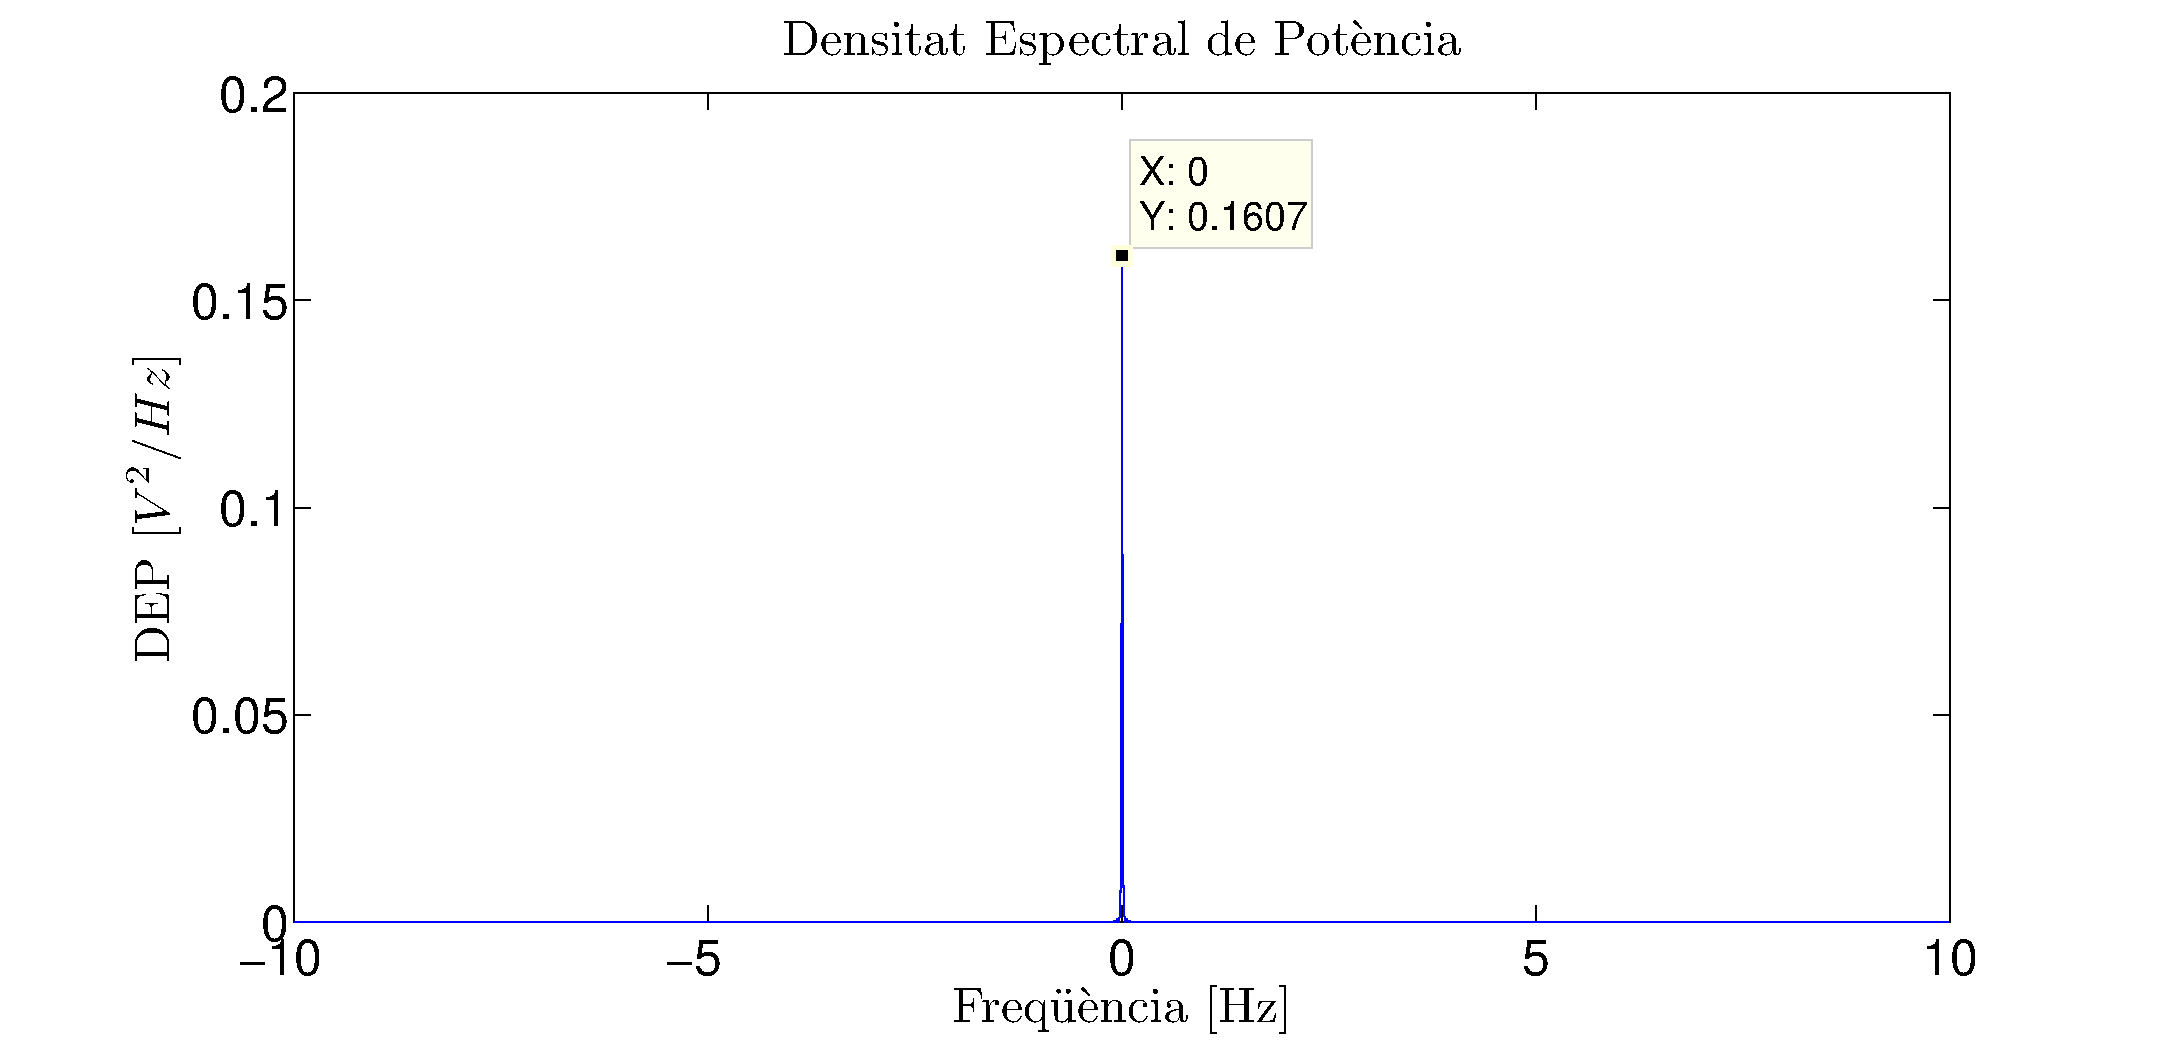
\includegraphics[width=0.8\textwidth]{Imatges/power_spectral_mean.eps}
\caption{Densitat espectral de la senyal $V_1$, amb una referència constant\label{fig:power_spectral_mean}}
\end{figure}

\begin{figure}[h]
\centering
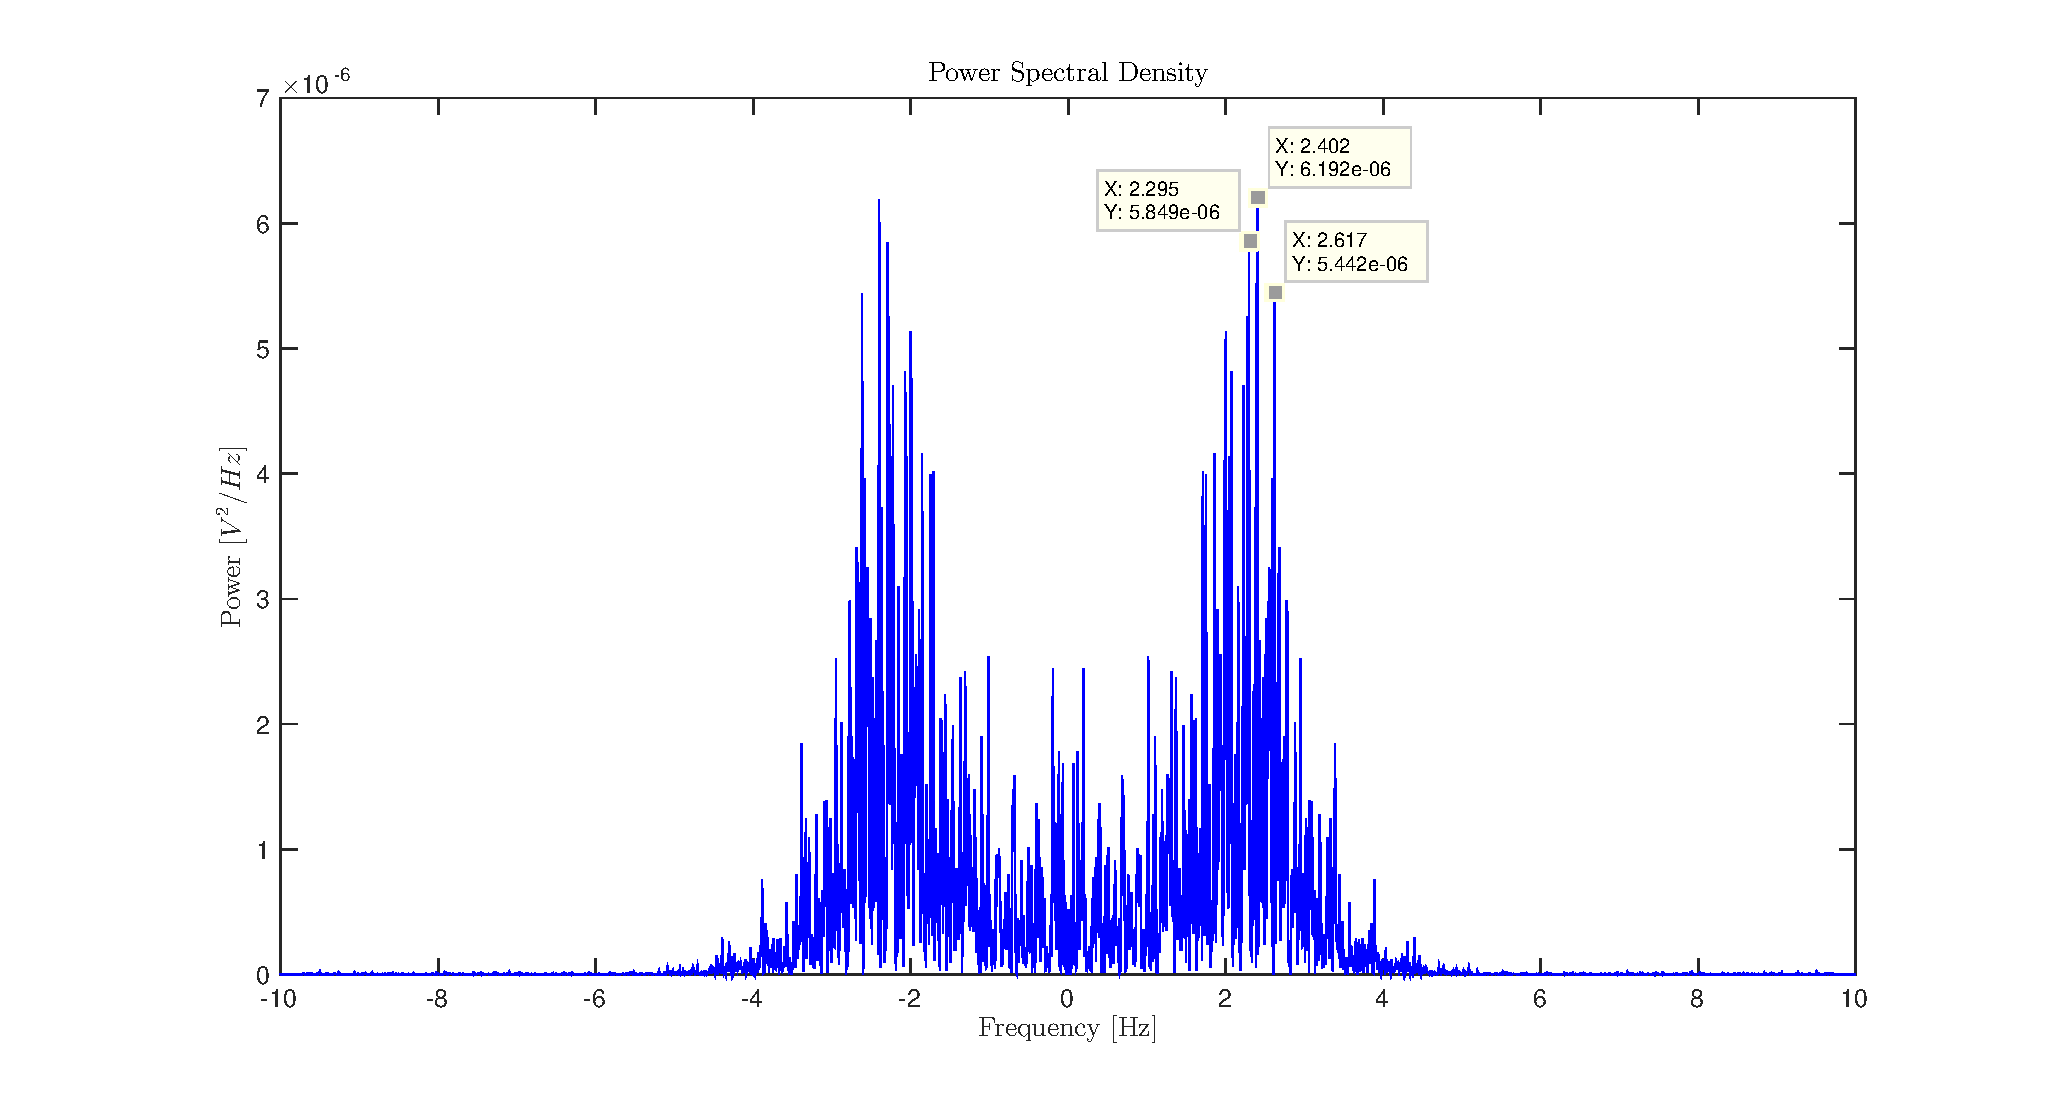
\includegraphics[width=0.8\textwidth]{Imatges/power_spectral_nomean_bef_sin_pols_imag.eps}
\caption{Densitat espectral de la senyal $V_1$ menys la mitja, amb una referència constant\label{fig:power_spectral_nomean_bef_sin_pols_imag}}
\end{figure}

\vspace{100pt}
Un cop escollida la freqüència a refusar, s'han de plantejar les matrius $\Phi_w$, $\Gamma_w$ i $C_w$ que modelen la pertorbació constant i sinusoïdal. El cas de la constant, s'ha definit el seu model en \eqref{eq:pert_const}. Per altra banda, el d'una sinusoïdal, en continu, és \eqref{eq:pert_sin_cont}, depenent de la freqüència $w_0$ expressada en radians per segon. Cal a dir, que la freqüència que s'ha escollit de $2.4$ és en unitats de Hz, per tant $w_0=2.4\cdot2\pi = 15.07964~\mathrm{\frac{rad}{s}}$. Ara bé, per a ser utilitzat, s'ha de passar a discret amb l'ús de $\Phi_{w_2}=e^{F_{w_2} T_s}$, sent el període de mostratge $T_s=0.05$ s.\footnote{Al llarg de l'informe es fa referència a les matrius corresponents a les pertorbacions constants amb el subíndex $w_1$ i a les de les pertorbacions sinusoïdals amb subíndex $w_2$.}

\begin{equation}\label{eq:pert_sin_cont}
\begin{bmatrix}
\dot{w}\\
\ddot{w}
\end{bmatrix} = \begin{bmatrix}
0 & 1\\
w_0^2 & 0
\end{bmatrix} \begin{bmatrix}
w\\
\dot{w}
\end{bmatrix} = F_{w_2} \begin{bmatrix}
w\\
\dot{w}
\end{bmatrix}
\end{equation}

Per tant, si s'acoblen les diferents matrius de les pertorbacions constants i sinusoïdals, dona com a resultat el model del sistema expressat en les equacions \eqref{eq:pert_sin_ct_model_mat}. En el moment que es tenen les matrius $\Phi_w$, $\Gamma_w$ i $C_w$ ja es pot utilitzar la formula d'Ackermann per calcular $L$, amb resultat expressat en \eqref{eq:pert_sin_ct_L}, i les equacions \eqref{eq:pert_model_glob} per definir l'observador.


\begin{equation}\label{eq:pert_sin_ct_model_mat}
\left\{
\begin{array}{lr}
\begin{bmatrix}
x_{k+1}\\
w_{k+1}^{d_1}\\
w_{k+1}^{d_2}\\
\dot{w}_{k+1}^{d_2}
\end{bmatrix} = 
\begin{bmatrix}
\Phi & \Gamma & \Gamma & 0\\
0 & 1 & 0 & 0\\
0 & 0 & a_{11} & a_{12}\\
0 & 0 & a_{21} & a_{22}
\end{bmatrix} \begin{bmatrix}
x_{k}\\
w_k^{d_1}\\
w_k^{d_2}\\
\dot{w}_k^{d_2}
\end{bmatrix} + 
\begin{bmatrix}
\Gamma\\
0\\
0\\
0
\end{bmatrix} u_k\\

y_k=\begin{bmatrix}
C & 0 & 0 & 0
\end{bmatrix} \begin{bmatrix}
x_{k}\\
w_k^{d_1}\\
w_k^{d_2}\\
\dot{w}_k^{d_2}
\end{bmatrix}\\

\Phi_{w_2}=\begin{bmatrix}
a_{11} & a_{12}\\
a_{21} & a_{22}
\end{bmatrix} = \begin{bmatrix}
0,72897 & 0,045395\\
-10,3227 & 0,72897
\end{bmatrix}

\end{array}
\right.
\end{equation}

\begin{equation}\label{eq:pert_sin_ct_L}
L=\begin{bmatrix}
2,10252\\
-1,08740\\
0,03339\\
-0,08400\\
-4,93555
\end{bmatrix}
\end{equation}


A l'hora de simular amb \texttt{Simulink} prenem el model \eqref{fig:pert_sim}, amb els nous valors de $\Phi_w$, $\Gamma_w$, $C_w$ i $L$ i fent les petites adaptacions de la realimentació d'estat observat i del \textit{feedforward} s'aconsegueix dur a terme la simulació.

La primera simulació que es prova és amb les pertorbacions constants (\textit{step}) i sinusoïdals. D'aquesta forma es comprova si refusa aquestes pertorbacions com es veu en la figura \ref{fig:pert_sin_ct_sim_pols_imag_no_soroll}. Per tant la funció principal d'aquest control es compleix de forma satisfactòria.

\begin{figure}[h]
\centering
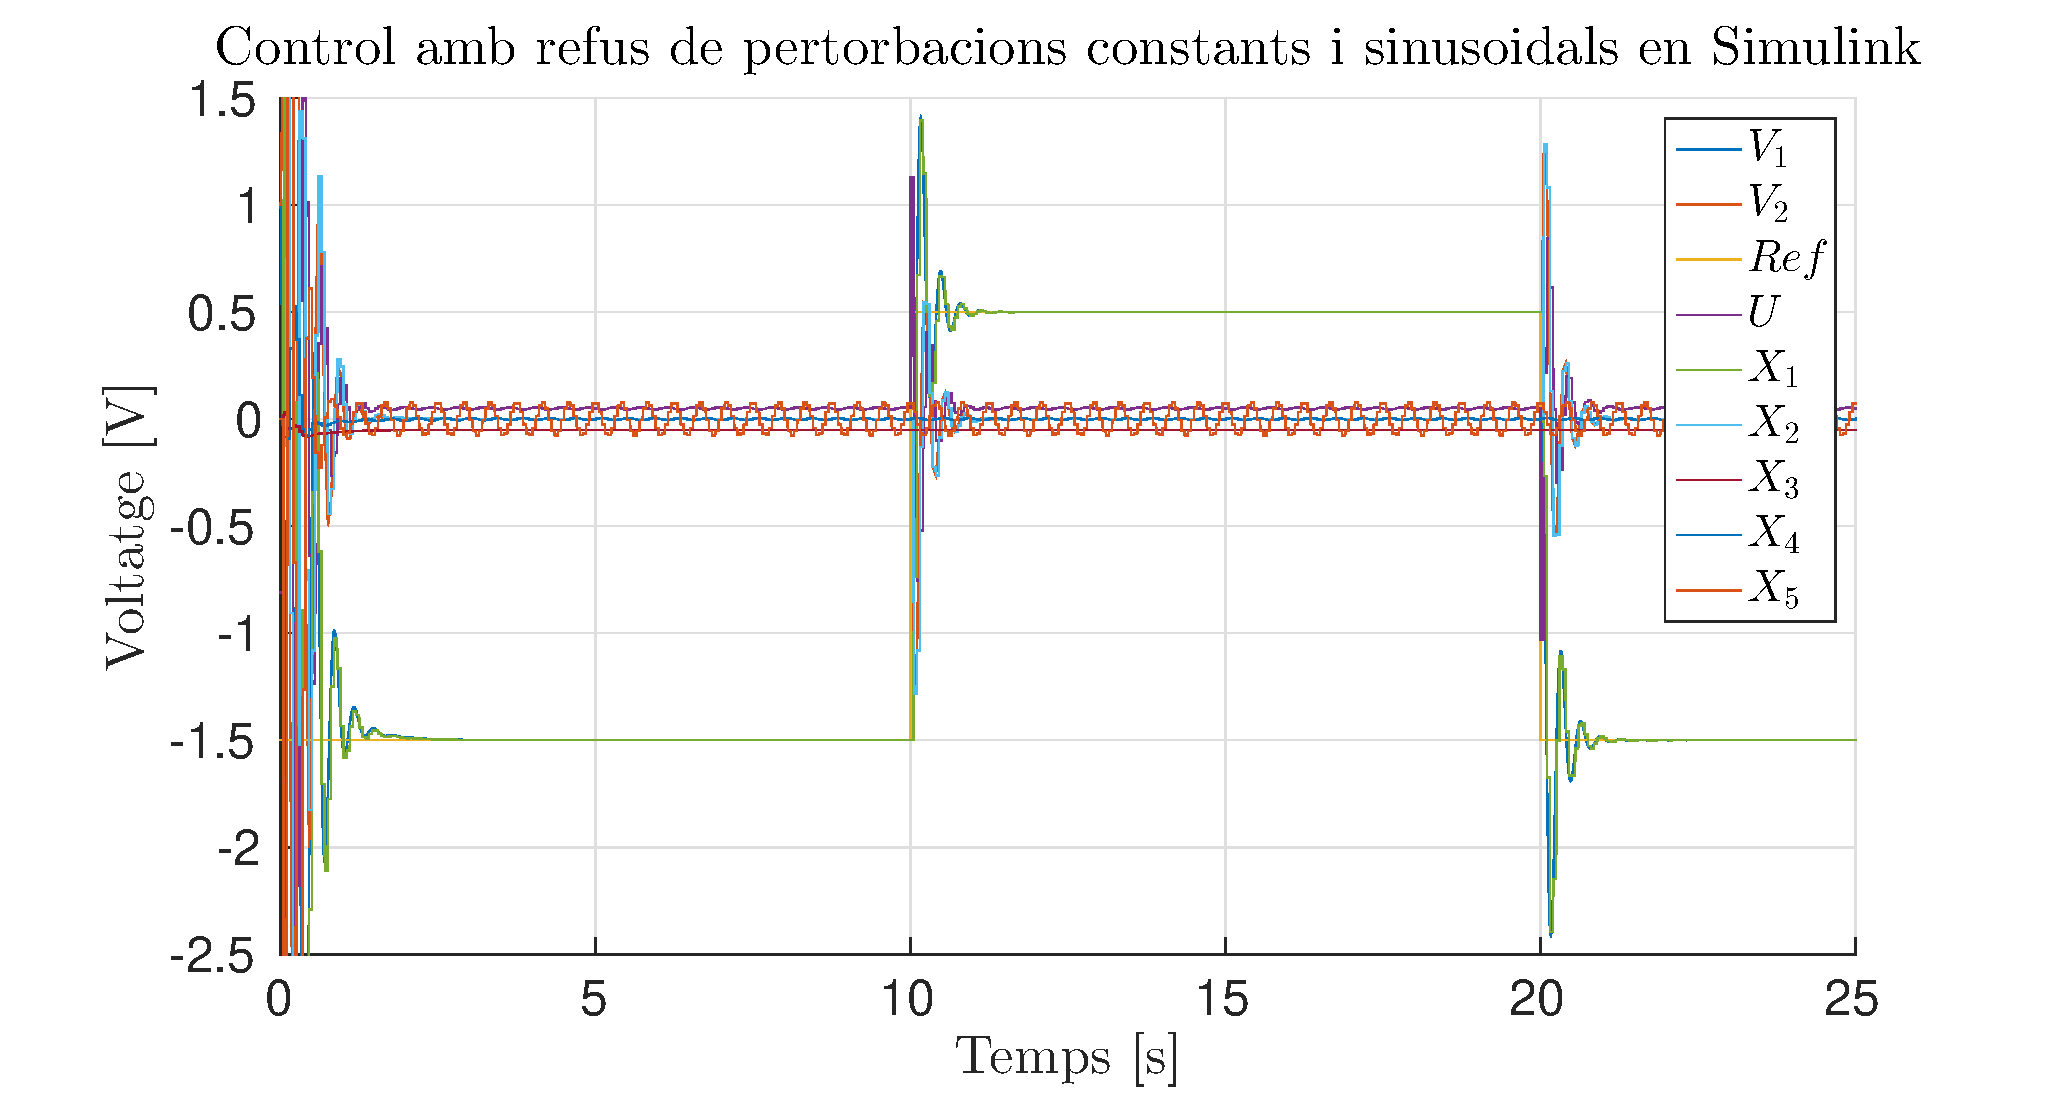
\includegraphics[width=0.8\textwidth]{Imatges/pert_sin_ct_sim_pols_imag_no_soroll.eps}
\caption{Dades de la simulació amb control amb refús de pertorbacions constants i sinusoïdals amb un \textit{step} i una sinusoïdal\label{fig:pert_sin_ct_sim_pols_imag_no_soroll}}
\end{figure}

Posteriorment, es prova afegint una pertorbació de soroll blanc, que intenta representar part del soroll real de la planta o els sensors. En aquest cas, representat en la figura \ref{fig:pert_sin_ct_sim_pols_imag_soroll}, el control no es capaç d'eliminar el soroll, ja que aquest no és ni un \textit{offset}, ni tampoc és una sinusoïdal de la freqüència refusada, per aconseguir-ho es requeriria d'un altre tipus de control, com podria ser el de refús de pertorbacions d'un rang de sinusoïdals.

\begin{figure}[h]
\centering
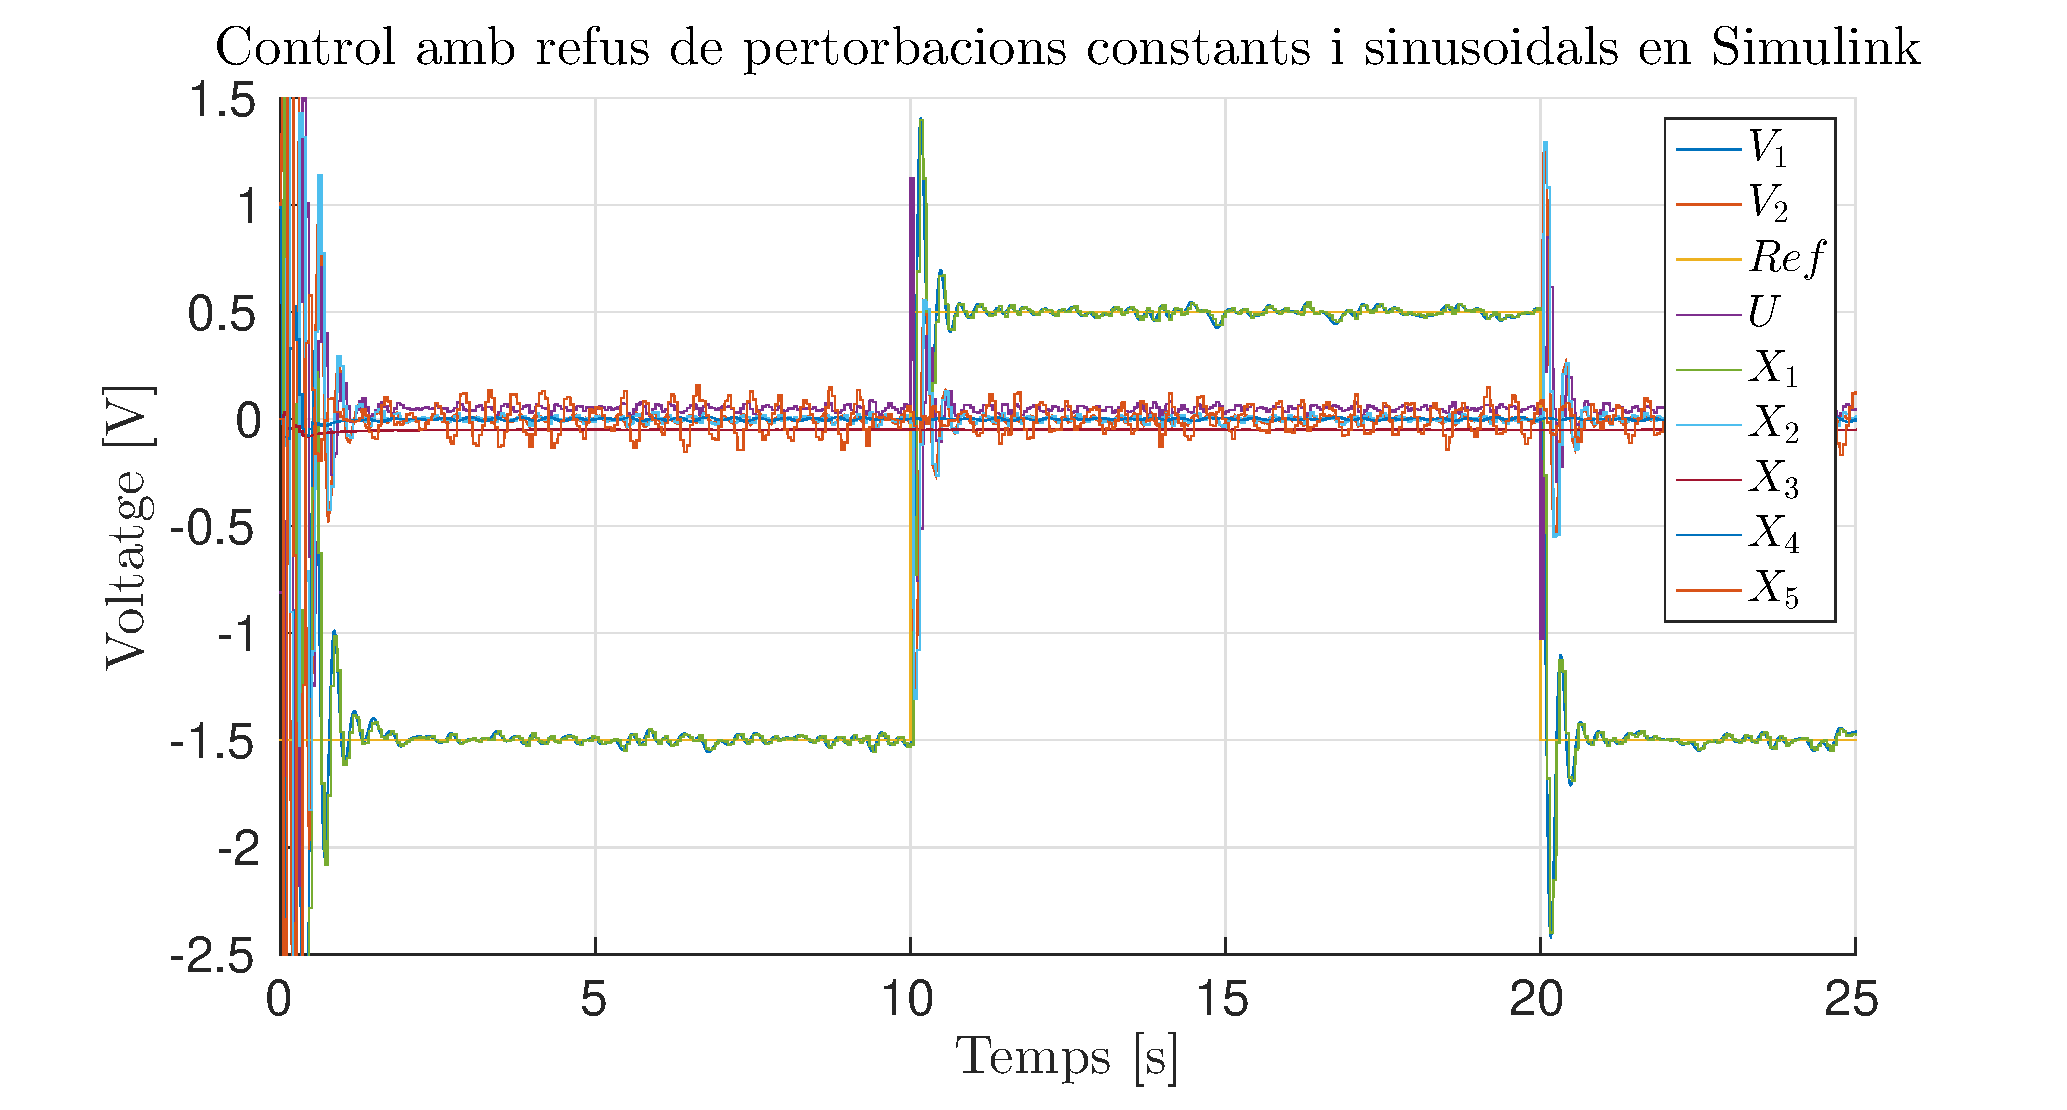
\includegraphics[width=0.8\textwidth]{Imatges/pert_sin_ct_sim_pols_imag_soroll.eps}
\caption{Dades de la simulació amb control amb refús de pertorbacions constants i sinusoïdals amb un \textit{step}, una sinusoïdal i soroll blanc\label{fig:pert_sin_ct_sim_pols_imag_soroll}}
\end{figure}

Un cop s'ha comprovat en la simulació que el control funciona de la forma desitjada, es pot procedir a la implementació en l'Arduino. En aquest cas en diferència al control de pertorbacions constants, només es diferencia en les matrius utilitzades i que en el \textit{feedforward} s'ha d'afegir el terme $w_k^{d_2}$, que correspon a l'estimació de la sinusoïdal. 

\vspace{16pt}
El resultat de la implementació és el de la figura \ref{fig:pert_sin_ct_pols_imag}, es veu com hi ha encara soroll, però el de freqüència $2.4$ Hz ha desaparegut. Aquest fet es pot comprovar millor observant el gràfic de la densitat espectral de potència, de la figura \ref{fig:power_spectral_nomean_pert_sin_pols_imag}. Ara bé, es cert que en $2.4$ Hz pràcticament no hi ha senyal, però s'ha intensificat en altres freqüències quedant en més o menys la mateixa potència. Per tant, es podria dir que aquest tipus de refús, per eliminar soroll general\footnote{Amb soroll general es refereix a que el soroll que es vol refusar no es degut a una causa concreta, i que per tant, no només treballa en una freqüència determinada.} provoca la distribució de la potència del soroll en altres freqüències.

\begin{figure}[h]
\centering
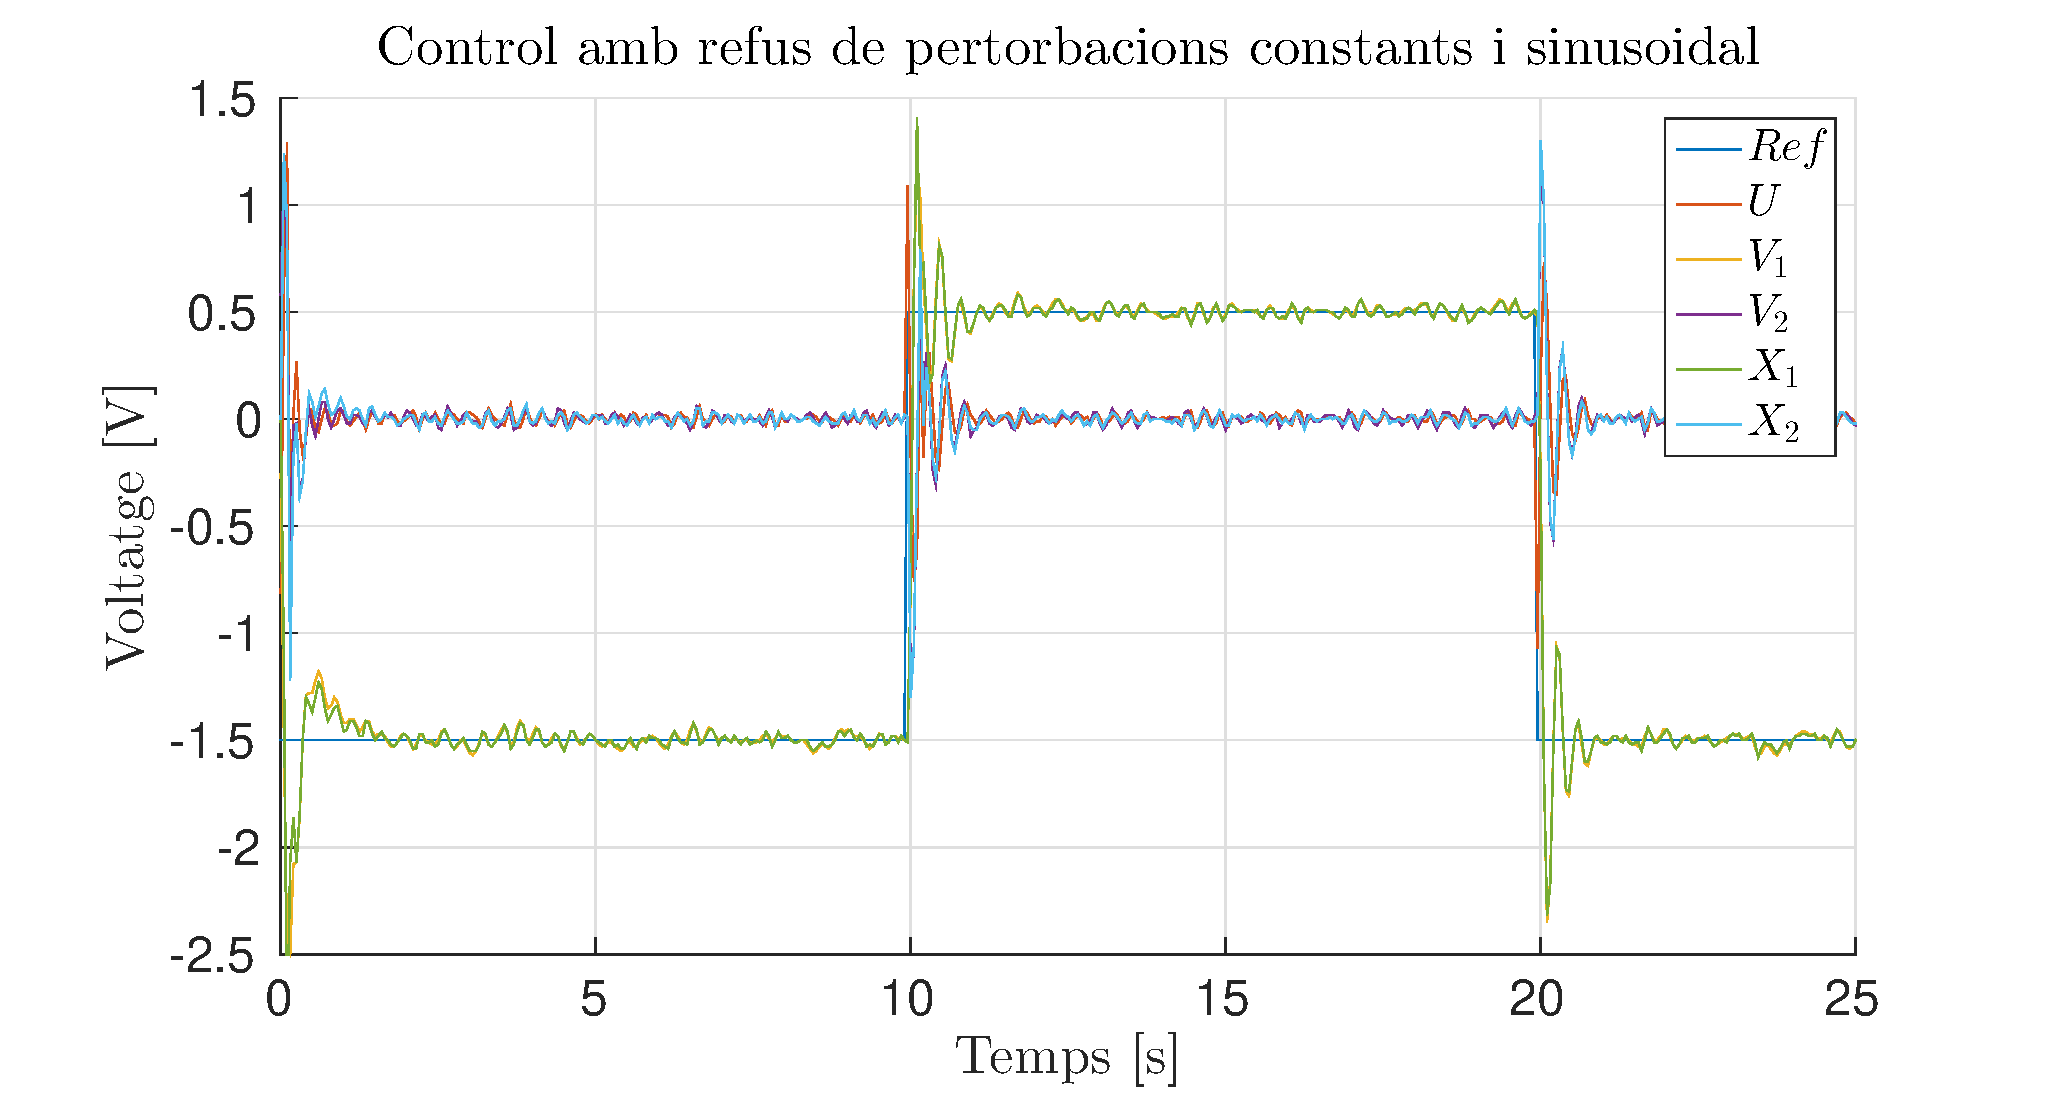
\includegraphics[width=0.8\textwidth]{Imatges/pert_sin_ct_pols_imag.eps}
\caption{Dades de l'Arduino amb control amb refús de pertorbacions constants i sinusoïdals\label{fig:pert_sin_ct_pols_imag}}
\end{figure}

\begin{figure}[h]
\centering
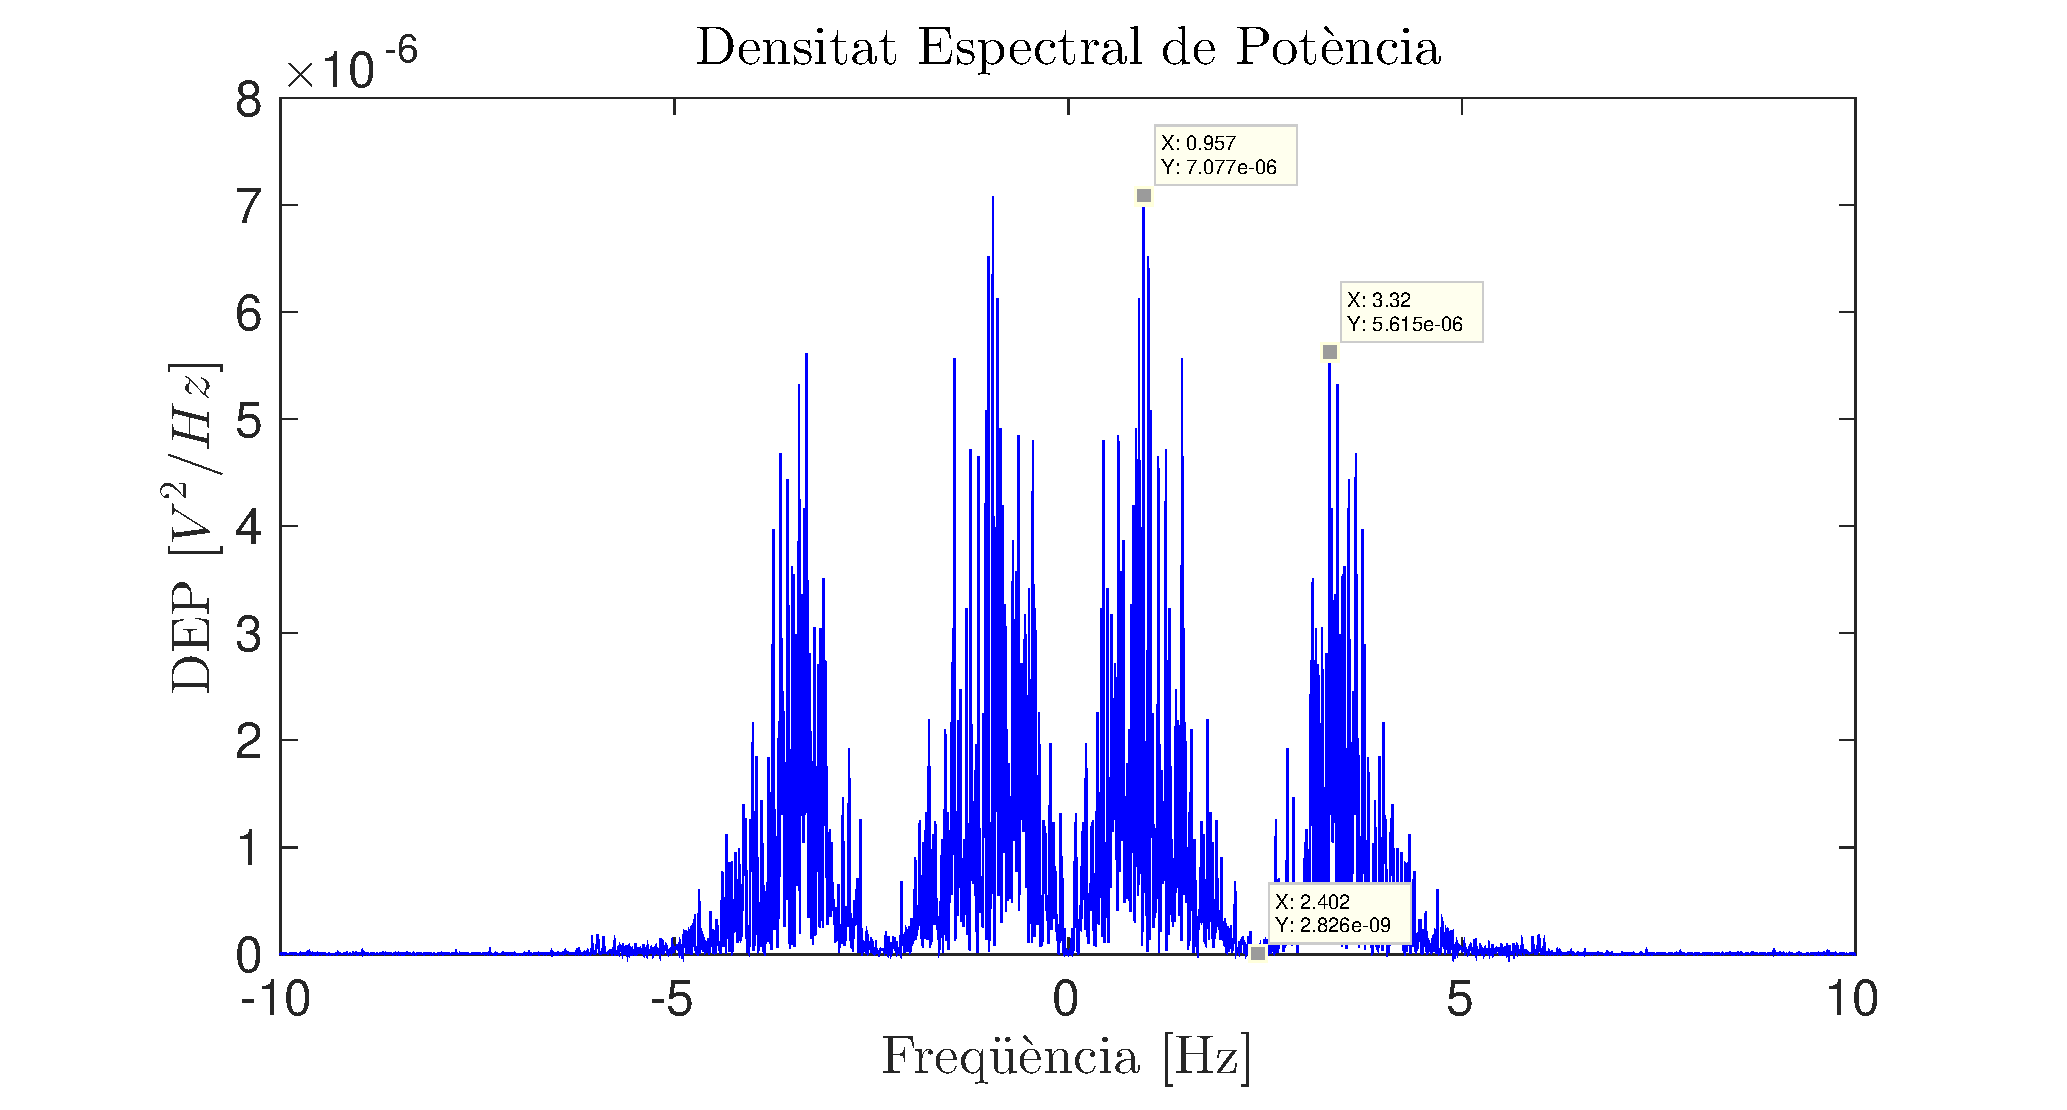
\includegraphics[width=0.8\textwidth]{Imatges/power_spectral_nomean_pert_sin_pols_imag.eps}
\caption{Densitat espectral de la senyal $V_1$, sense els transitoris i menys la mitja en cada tram, del control amb refús de pertorbacions constants i sinusoïdals\label{fig:power_spectral_nomean_pert_sin_pols_imag}}
\end{figure}


%Dir que amb el fet de posar refusar a una certa frequencia la potencia es distribueix en altres frequencies
\subsection{Pertorbacions d'un rang de freqüències sinusoïdals}
\label{sec:pert_rang_sin}

\section{Ús de pols reals de l'observador}
%S'ha vist que hi ha unes freqüencies molt altes i s'ha pensat en que poden ser degudes als pols de l'observador que s'han posat, per això es decideix a procedir amb l'ús de pols reals en lloc dels proposats a l'inici.
%Després també es veu com el fet que siguin ràpids no es necessari ja que es preten refusar un senyal que es sempre igual. Es veu en la transformada de fourier.

%\bibliography{./Bibliografia/library}
%\addcontentsline{toc}{chapter}{Referències}
%\label{Referencies}


\appendix
\clearpage % o \cleardoublepage
\addappheadtotoc
\appendixpage

\chapter{Càlculs per refús de pertorbacions d'un rang de freqüències sinusoïdals}

\end{document}
